% Options for packages loaded elsewhere
\PassOptionsToPackage{unicode}{hyperref}
\PassOptionsToPackage{hyphens}{url}
\PassOptionsToPackage{dvipsnames,svgnames,x11names}{xcolor}
%
\documentclass[
  letterpaper,
  DIV=11,
  numbers=noendperiod]{scrartcl}

\usepackage{amsmath,amssymb}
\usepackage{iftex}
\ifPDFTeX
  \usepackage[T1]{fontenc}
  \usepackage[utf8]{inputenc}
  \usepackage{textcomp} % provide euro and other symbols
\else % if luatex or xetex
  \usepackage{unicode-math}
  \defaultfontfeatures{Scale=MatchLowercase}
  \defaultfontfeatures[\rmfamily]{Ligatures=TeX,Scale=1}
\fi
\usepackage{lmodern}
\ifPDFTeX\else  
    % xetex/luatex font selection
\fi
% Use upquote if available, for straight quotes in verbatim environments
\IfFileExists{upquote.sty}{\usepackage{upquote}}{}
\IfFileExists{microtype.sty}{% use microtype if available
  \usepackage[]{microtype}
  \UseMicrotypeSet[protrusion]{basicmath} % disable protrusion for tt fonts
}{}
\makeatletter
\@ifundefined{KOMAClassName}{% if non-KOMA class
  \IfFileExists{parskip.sty}{%
    \usepackage{parskip}
  }{% else
    \setlength{\parindent}{0pt}
    \setlength{\parskip}{6pt plus 2pt minus 1pt}}
}{% if KOMA class
  \KOMAoptions{parskip=half}}
\makeatother
\usepackage{xcolor}
\setlength{\emergencystretch}{3em} % prevent overfull lines
\setcounter{secnumdepth}{5}
% Make \paragraph and \subparagraph free-standing
\ifx\paragraph\undefined\else
  \let\oldparagraph\paragraph
  \renewcommand{\paragraph}[1]{\oldparagraph{#1}\mbox{}}
\fi
\ifx\subparagraph\undefined\else
  \let\oldsubparagraph\subparagraph
  \renewcommand{\subparagraph}[1]{\oldsubparagraph{#1}\mbox{}}
\fi

\usepackage{color}
\usepackage{fancyvrb}
\newcommand{\VerbBar}{|}
\newcommand{\VERB}{\Verb[commandchars=\\\{\}]}
\DefineVerbatimEnvironment{Highlighting}{Verbatim}{commandchars=\\\{\}}
% Add ',fontsize=\small' for more characters per line
\usepackage{framed}
\definecolor{shadecolor}{RGB}{241,243,245}
\newenvironment{Shaded}{\begin{snugshade}}{\end{snugshade}}
\newcommand{\AlertTok}[1]{\textcolor[rgb]{0.68,0.00,0.00}{#1}}
\newcommand{\AnnotationTok}[1]{\textcolor[rgb]{0.37,0.37,0.37}{#1}}
\newcommand{\AttributeTok}[1]{\textcolor[rgb]{0.40,0.45,0.13}{#1}}
\newcommand{\BaseNTok}[1]{\textcolor[rgb]{0.68,0.00,0.00}{#1}}
\newcommand{\BuiltInTok}[1]{\textcolor[rgb]{0.00,0.23,0.31}{#1}}
\newcommand{\CharTok}[1]{\textcolor[rgb]{0.13,0.47,0.30}{#1}}
\newcommand{\CommentTok}[1]{\textcolor[rgb]{0.37,0.37,0.37}{#1}}
\newcommand{\CommentVarTok}[1]{\textcolor[rgb]{0.37,0.37,0.37}{\textit{#1}}}
\newcommand{\ConstantTok}[1]{\textcolor[rgb]{0.56,0.35,0.01}{#1}}
\newcommand{\ControlFlowTok}[1]{\textcolor[rgb]{0.00,0.23,0.31}{#1}}
\newcommand{\DataTypeTok}[1]{\textcolor[rgb]{0.68,0.00,0.00}{#1}}
\newcommand{\DecValTok}[1]{\textcolor[rgb]{0.68,0.00,0.00}{#1}}
\newcommand{\DocumentationTok}[1]{\textcolor[rgb]{0.37,0.37,0.37}{\textit{#1}}}
\newcommand{\ErrorTok}[1]{\textcolor[rgb]{0.68,0.00,0.00}{#1}}
\newcommand{\ExtensionTok}[1]{\textcolor[rgb]{0.00,0.23,0.31}{#1}}
\newcommand{\FloatTok}[1]{\textcolor[rgb]{0.68,0.00,0.00}{#1}}
\newcommand{\FunctionTok}[1]{\textcolor[rgb]{0.28,0.35,0.67}{#1}}
\newcommand{\ImportTok}[1]{\textcolor[rgb]{0.00,0.46,0.62}{#1}}
\newcommand{\InformationTok}[1]{\textcolor[rgb]{0.37,0.37,0.37}{#1}}
\newcommand{\KeywordTok}[1]{\textcolor[rgb]{0.00,0.23,0.31}{#1}}
\newcommand{\NormalTok}[1]{\textcolor[rgb]{0.00,0.23,0.31}{#1}}
\newcommand{\OperatorTok}[1]{\textcolor[rgb]{0.37,0.37,0.37}{#1}}
\newcommand{\OtherTok}[1]{\textcolor[rgb]{0.00,0.23,0.31}{#1}}
\newcommand{\PreprocessorTok}[1]{\textcolor[rgb]{0.68,0.00,0.00}{#1}}
\newcommand{\RegionMarkerTok}[1]{\textcolor[rgb]{0.00,0.23,0.31}{#1}}
\newcommand{\SpecialCharTok}[1]{\textcolor[rgb]{0.37,0.37,0.37}{#1}}
\newcommand{\SpecialStringTok}[1]{\textcolor[rgb]{0.13,0.47,0.30}{#1}}
\newcommand{\StringTok}[1]{\textcolor[rgb]{0.13,0.47,0.30}{#1}}
\newcommand{\VariableTok}[1]{\textcolor[rgb]{0.07,0.07,0.07}{#1}}
\newcommand{\VerbatimStringTok}[1]{\textcolor[rgb]{0.13,0.47,0.30}{#1}}
\newcommand{\WarningTok}[1]{\textcolor[rgb]{0.37,0.37,0.37}{\textit{#1}}}

\providecommand{\tightlist}{%
  \setlength{\itemsep}{0pt}\setlength{\parskip}{0pt}}\usepackage{longtable,booktabs,array}
\usepackage{calc} % for calculating minipage widths
% Correct order of tables after \paragraph or \subparagraph
\usepackage{etoolbox}
\makeatletter
\patchcmd\longtable{\par}{\if@noskipsec\mbox{}\fi\par}{}{}
\makeatother
% Allow footnotes in longtable head/foot
\IfFileExists{footnotehyper.sty}{\usepackage{footnotehyper}}{\usepackage{footnote}}
\makesavenoteenv{longtable}
\usepackage{graphicx}
\makeatletter
\def\maxwidth{\ifdim\Gin@nat@width>\linewidth\linewidth\else\Gin@nat@width\fi}
\def\maxheight{\ifdim\Gin@nat@height>\textheight\textheight\else\Gin@nat@height\fi}
\makeatother
% Scale images if necessary, so that they will not overflow the page
% margins by default, and it is still possible to overwrite the defaults
% using explicit options in \includegraphics[width, height, ...]{}
\setkeys{Gin}{width=\maxwidth,height=\maxheight,keepaspectratio}
% Set default figure placement to htbp
\makeatletter
\def\fps@figure{htbp}
\makeatother
\newlength{\cslhangindent}
\setlength{\cslhangindent}{1.5em}
\newlength{\csllabelwidth}
\setlength{\csllabelwidth}{3em}
\newlength{\cslentryspacingunit} % times entry-spacing
\setlength{\cslentryspacingunit}{\parskip}
\newenvironment{CSLReferences}[2] % #1 hanging-ident, #2 entry spacing
 {% don't indent paragraphs
  \setlength{\parindent}{0pt}
  % turn on hanging indent if param 1 is 1
  \ifodd #1
  \let\oldpar\par
  \def\par{\hangindent=\cslhangindent\oldpar}
  \fi
  % set entry spacing
  \setlength{\parskip}{#2\cslentryspacingunit}
 }%
 {}
\usepackage{calc}
\newcommand{\CSLBlock}[1]{#1\hfill\break}
\newcommand{\CSLLeftMargin}[1]{\parbox[t]{\csllabelwidth}{#1}}
\newcommand{\CSLRightInline}[1]{\parbox[t]{\linewidth - \csllabelwidth}{#1}\break}
\newcommand{\CSLIndent}[1]{\hspace{\cslhangindent}#1}

\usepackage{booktabs}
\usepackage{longtable}
\usepackage{array}
\usepackage{multirow}
\usepackage{wrapfig}
\usepackage{float}
\usepackage{colortbl}
\usepackage{pdflscape}
\usepackage{tabu}
\usepackage{threeparttable}
\usepackage{threeparttablex}
\usepackage[normalem]{ulem}
\usepackage{makecell}
\usepackage{xcolor}
\usepackage{siunitx}

  \newcolumntype{d}{S[
    input-open-uncertainty=,
    input-close-uncertainty=,
    parse-numbers = false,
    table-align-text-pre=false,
    table-align-text-post=false
  ]}
  
\KOMAoption{captions}{tableheading}
\makeatletter
\makeatother
\makeatletter
\makeatother
\makeatletter
\@ifpackageloaded{caption}{}{\usepackage{caption}}
\AtBeginDocument{%
\ifdefined\contentsname
  \renewcommand*\contentsname{Table of contents}
\else
  \newcommand\contentsname{Table of contents}
\fi
\ifdefined\listfigurename
  \renewcommand*\listfigurename{List of Figures}
\else
  \newcommand\listfigurename{List of Figures}
\fi
\ifdefined\listtablename
  \renewcommand*\listtablename{List of Tables}
\else
  \newcommand\listtablename{List of Tables}
\fi
\ifdefined\figurename
  \renewcommand*\figurename{Figure}
\else
  \newcommand\figurename{Figure}
\fi
\ifdefined\tablename
  \renewcommand*\tablename{Table}
\else
  \newcommand\tablename{Table}
\fi
}
\@ifpackageloaded{float}{}{\usepackage{float}}
\floatstyle{ruled}
\@ifundefined{c@chapter}{\newfloat{codelisting}{h}{lop}}{\newfloat{codelisting}{h}{lop}[chapter]}
\floatname{codelisting}{Listing}
\newcommand*\listoflistings{\listof{codelisting}{List of Listings}}
\makeatother
\makeatletter
\@ifpackageloaded{caption}{}{\usepackage{caption}}
\@ifpackageloaded{subcaption}{}{\usepackage{subcaption}}
\makeatother
\makeatletter
\@ifpackageloaded{tcolorbox}{}{\usepackage[skins,breakable]{tcolorbox}}
\makeatother
\makeatletter
\@ifundefined{shadecolor}{\definecolor{shadecolor}{rgb}{.97, .97, .97}}
\makeatother
\makeatletter
\makeatother
\makeatletter
\makeatother
\ifLuaTeX
  \usepackage{selnolig}  % disable illegal ligatures
\fi
\IfFileExists{bookmark.sty}{\usepackage{bookmark}}{\usepackage{hyperref}}
\IfFileExists{xurl.sty}{\usepackage{xurl}}{} % add URL line breaks if available
\urlstyle{same} % disable monospaced font for URLs
\hypersetup{
  pdftitle={My title},
  pdfauthor={Hannah Yu},
  colorlinks=true,
  linkcolor={blue},
  filecolor={Maroon},
  citecolor={Blue},
  urlcolor={Blue},
  pdfcreator={LaTeX via pandoc}}

\title{My title\thanks{Code and data are available at: LINK.}}
\usepackage{etoolbox}
\makeatletter
\providecommand{\subtitle}[1]{% add subtitle to \maketitle
  \apptocmd{\@title}{\par {\large #1 \par}}{}{}
}
\makeatother
\subtitle{My subtitle if needed}
\author{Hannah Yu}
\date{April 11, 2024}

\begin{document}
\maketitle
\begin{abstract}
First sentence. Second sentence. Third sentence. Fourth sentence.
\end{abstract}
\ifdefined\Shaded\renewenvironment{Shaded}{\begin{tcolorbox}[enhanced, sharp corners, frame hidden, borderline west={3pt}{0pt}{shadecolor}, interior hidden, boxrule=0pt, breakable]}{\end{tcolorbox}}\fi

\begin{Shaded}
\begin{Highlighting}[]
\NormalTok{ces2020 }\OtherTok{\textless{}{-}}  \FunctionTok{read\_parquet}\NormalTok{(here}\SpecialCharTok{::}\FunctionTok{here}\NormalTok{(}\StringTok{"data/analysis\_data/cleaned\_ces2020.parquet"}\NormalTok{))}
\end{Highlighting}
\end{Shaded}

\hypertarget{introduction}{%
\section{Introduction}\label{introduction}}

You can and should cross-reference sections and sub-sections. We use R
Core Team (2023) and Wickham et al. (2019).

The remainder of this paper is structured as follows.
Section~\ref{sec-data}\ldots.

\hypertarget{sec-data}{%
\section{Data}\label{sec-data}}

Data analysis is performed using statistical programming language R (R
Core Team 2023), with packages \texttt{tidyverse}
(\textbf{citeTidyverse?}), \texttt{here} (\textbf{citeHere?}),
\texttt{rstanarm} (\textbf{citeRstanarm?}), \texttt{modelsummary}
(\textbf{citeModleSummary?}), \texttt{ggplot2} (\textbf{citeGgplot2?}),
\texttt{knitr} (\textbf{citeKnitr?}), \texttt{marginaleffects}
(\textbf{citeMarginalEffects?}), \texttt{plotly} (\textbf{citePlotly?}),
\texttt{tibble} (\textbf{citeTibble?}), \texttt{margins}
(\textbf{citeMargins?}), \texttt{testthat} (\textbf{citetestthat?}) and
\texttt{kableExtra} (\textbf{citeKableExtra?}).

\hypertarget{data-source}{%
\subsection{Data Source}\label{data-source}}

Data for this research comes from the 2020 Cooperative Election Study
(CES) (\textbf{citeCes2020?}), a annual US political survey. The CES
contains information about Americans' political view, voting behaviours
and experiences across various political geography and social context.
61,000 American adults participated in the survey in 2020.

\hypertarget{data-cleaning-and-variables}{%
\subsection{Data Cleaning and
Variables}\label{data-cleaning-and-variables}}

\hypertarget{tbl-clean-data}{}
\begin{longtable}[]{@{}
  >{\raggedright\arraybackslash}p{(\columnwidth - 20\tabcolsep) * \real{0.1408}}
  >{\raggedright\arraybackslash}p{(\columnwidth - 20\tabcolsep) * \real{0.0563}}
  >{\raggedright\arraybackslash}p{(\columnwidth - 20\tabcolsep) * \real{0.0563}}
  >{\raggedright\arraybackslash}p{(\columnwidth - 20\tabcolsep) * \real{0.0563}}
  >{\raggedright\arraybackslash}p{(\columnwidth - 20\tabcolsep) * \real{0.0563}}
  >{\raggedright\arraybackslash}p{(\columnwidth - 20\tabcolsep) * \real{0.1268}}
  >{\raggedright\arraybackslash}p{(\columnwidth - 20\tabcolsep) * \real{0.0845}}
  >{\raggedright\arraybackslash}p{(\columnwidth - 20\tabcolsep) * \real{0.0563}}
  >{\raggedright\arraybackslash}p{(\columnwidth - 20\tabcolsep) * \real{0.0845}}
  >{\raggedright\arraybackslash}p{(\columnwidth - 20\tabcolsep) * \real{0.1127}}
  >{\raggedright\arraybackslash}p{(\columnwidth - 20\tabcolsep) * \real{0.1690}}@{}}
\caption{\label{tbl-clean-data}Preview of the cleaned 2020 CES
dataset}\tabularnewline
\toprule\noalign{}
\begin{minipage}[b]{\linewidth}\raggedright
voted\_for
\end{minipage} & \begin{minipage}[b]{\linewidth}\raggedright
ABC
\end{minipage} & \begin{minipage}[b]{\linewidth}\raggedright
CBS
\end{minipage} & \begin{minipage}[b]{\linewidth}\raggedright
NBC
\end{minipage} & \begin{minipage}[b]{\linewidth}\raggedright
CNN
\end{minipage} & \begin{minipage}[b]{\linewidth}\raggedright
Fox\_News
\end{minipage} & \begin{minipage}[b]{\linewidth}\raggedright
MSNBC
\end{minipage} & \begin{minipage}[b]{\linewidth}\raggedright
PBS
\end{minipage} & \begin{minipage}[b]{\linewidth}\raggedright
Other
\end{minipage} & \begin{minipage}[b]{\linewidth}\raggedright
TV\_type
\end{minipage} & \begin{minipage}[b]{\linewidth}\raggedright
Party
\end{minipage} \\
\midrule\noalign{}
\endfirsthead
\toprule\noalign{}
\begin{minipage}[b]{\linewidth}\raggedright
voted\_for
\end{minipage} & \begin{minipage}[b]{\linewidth}\raggedright
ABC
\end{minipage} & \begin{minipage}[b]{\linewidth}\raggedright
CBS
\end{minipage} & \begin{minipage}[b]{\linewidth}\raggedright
NBC
\end{minipage} & \begin{minipage}[b]{\linewidth}\raggedright
CNN
\end{minipage} & \begin{minipage}[b]{\linewidth}\raggedright
Fox\_News
\end{minipage} & \begin{minipage}[b]{\linewidth}\raggedright
MSNBC
\end{minipage} & \begin{minipage}[b]{\linewidth}\raggedright
PBS
\end{minipage} & \begin{minipage}[b]{\linewidth}\raggedright
Other
\end{minipage} & \begin{minipage}[b]{\linewidth}\raggedright
TV\_type
\end{minipage} & \begin{minipage}[b]{\linewidth}\raggedright
Party
\end{minipage} \\
\midrule\noalign{}
\endhead
\bottomrule\noalign{}
\endlastfoot
Trump & Yes & Yes & Yes & Yes & Yes & No & No & No & Both &
Republican \\
Biden & Yes & Yes & Yes & No & No & Yes & No & No & Both &
Independent \\
Biden & Yes & No & No & No & No & No & No & No & Both & Independent \\
Trump & No & No & No & No & Yes & Yes & No & No & Both & Republican \\
Biden & No & No & Yes & Yes & No & Yes & No & No & Both & Democrat \\
\end{longtable}

\hypertarget{tbl-summary}{}
\begin{longtable}[]{@{}
  >{\raggedright\arraybackslash}p{(\columnwidth - 22\tabcolsep) * \real{0.0221}}
  >{\raggedright\arraybackslash}p{(\columnwidth - 22\tabcolsep) * \real{0.0882}}
  >{\raggedright\arraybackslash}p{(\columnwidth - 22\tabcolsep) * \real{0.0735}}
  >{\raggedright\arraybackslash}p{(\columnwidth - 22\tabcolsep) * \real{0.0735}}
  >{\raggedright\arraybackslash}p{(\columnwidth - 22\tabcolsep) * \real{0.0735}}
  >{\raggedright\arraybackslash}p{(\columnwidth - 22\tabcolsep) * \real{0.0735}}
  >{\raggedright\arraybackslash}p{(\columnwidth - 22\tabcolsep) * \real{0.0735}}
  >{\raggedright\arraybackslash}p{(\columnwidth - 22\tabcolsep) * \real{0.0735}}
  >{\raggedright\arraybackslash}p{(\columnwidth - 22\tabcolsep) * \real{0.0735}}
  >{\raggedright\arraybackslash}p{(\columnwidth - 22\tabcolsep) * \real{0.0735}}
  >{\raggedright\arraybackslash}p{(\columnwidth - 22\tabcolsep) * \real{0.1765}}
  >{\raggedright\arraybackslash}p{(\columnwidth - 22\tabcolsep) * \real{0.1250}}@{}}
\caption{\label{tbl-summary}Statistics summary of the cleaned 2020 CES
dataset}\tabularnewline
\toprule\noalign{}
\begin{minipage}[b]{\linewidth}\raggedright
\end{minipage} & \begin{minipage}[b]{\linewidth}\raggedright
voted\_for
\end{minipage} & \begin{minipage}[b]{\linewidth}\raggedright
ABC
\end{minipage} & \begin{minipage}[b]{\linewidth}\raggedright
CBS
\end{minipage} & \begin{minipage}[b]{\linewidth}\raggedright
NBC
\end{minipage} & \begin{minipage}[b]{\linewidth}\raggedright
CNN
\end{minipage} & \begin{minipage}[b]{\linewidth}\raggedright
Fox\_News
\end{minipage} & \begin{minipage}[b]{\linewidth}\raggedright
MSNBC
\end{minipage} & \begin{minipage}[b]{\linewidth}\raggedright
PBS
\end{minipage} & \begin{minipage}[b]{\linewidth}\raggedright
Other
\end{minipage} & \begin{minipage}[b]{\linewidth}\raggedright
TV\_type
\end{minipage} & \begin{minipage}[b]{\linewidth}\raggedright
Party
\end{minipage} \\
\midrule\noalign{}
\endfirsthead
\toprule\noalign{}
\begin{minipage}[b]{\linewidth}\raggedright
\end{minipage} & \begin{minipage}[b]{\linewidth}\raggedright
voted\_for
\end{minipage} & \begin{minipage}[b]{\linewidth}\raggedright
ABC
\end{minipage} & \begin{minipage}[b]{\linewidth}\raggedright
CBS
\end{minipage} & \begin{minipage}[b]{\linewidth}\raggedright
NBC
\end{minipage} & \begin{minipage}[b]{\linewidth}\raggedright
CNN
\end{minipage} & \begin{minipage}[b]{\linewidth}\raggedright
Fox\_News
\end{minipage} & \begin{minipage}[b]{\linewidth}\raggedright
MSNBC
\end{minipage} & \begin{minipage}[b]{\linewidth}\raggedright
PBS
\end{minipage} & \begin{minipage}[b]{\linewidth}\raggedright
Other
\end{minipage} & \begin{minipage}[b]{\linewidth}\raggedright
TV\_type
\end{minipage} & \begin{minipage}[b]{\linewidth}\raggedright
Party
\end{minipage} \\
\midrule\noalign{}
\endhead
\bottomrule\noalign{}
\endlastfoot
& Trump: 7884 & Yes: 7402 & Yes: 6650 & Yes: 7333 & Yes: 8311 & Yes:
8384 & No :14444 & No :18073 & No :19222 & Local Newscast : 0 & Democrat
:9819 \\
& Biden:13328 & No :13810 & No :14562 & No :13879 & No :12901 & No
:12828 & Yes: 6768 & Yes: 3139 & Yes: 1990 & National Newscast: 7422 &
Republican :5642 \\
& NA & NA & NA & NA & NA & NA & NA & NA & NA & Both :13790 &
Independent:5217 \\
& NA & NA & NA & NA & NA & NA & NA & NA & NA & NA & Other : 534 \\
\end{longtable}

Table~\ref{tbl-summary} presentts a summary of the cleaned data, showing
detailed statistics about the dataset. Iis evident that Biden has more
supporters in this election. The seven listed media networks capture the
majority networks people watch; while \texttt{Other} captures the rest.
Due to the small number of respondents that only watch local newscast,

As we can see from the table, there are more people who support Biden.
Respondents covered a wide range of races, with white people being the
most heavily represented. Also, CES data came from a variety of
locations, but the majority came from the southern region of the United
States. The employment status of those who completed the survey varied,
with most of them being full-time or retired.

Since this paper focuses on analyzing the influence of media usage on
registered voters decision, I perform the following data cleaning
process and selected the related variables. The dataset is cleaned by
renaming the column names, changing the variable for from categorical to
dummy, selecting the variables of interest, and filtering out missing
information and information not related to the study. After cleaning,
there are 10331 rows of data remain in the cleaned dataset.
Table~\ref{tbl-clean-data} shows a preview of the cleaned dataset.

The dependent variable of my examination is: \texttt{presvote20post},
renamed to \texttt{voted\_for}. This variable represents the
presidential candidate the respondent voted for in the 2020 election in
the form of a numerical variable. The variable \texttt{votereg}
represents whether the respondent is registered to vote using numerical
numbers. This paper will only analyze respondents who are registered to
vote and focus on the outcome of two candidates, Joe Biden representing
the Democratic party and Donald Trump representing the Republican party.
To analyze the observations of interest, I first limited the
observations to the ones that responded ``Yes'' in \texttt{votereg}. And
I filtered the responses in \texttt{presvote20post} to only ``Biden'' or
``Trump'' and converted the variable into a dummy variable where 1
represents ``Biden'' and 0 represents ``Trump''. Rest of the variable
this paper focuses on are being divided into three categories: Media Use
- Networks, Media Use - TV Type, and Party Affiliation.

Media Use - Networks:

\begin{itemize}
\item
  \texttt{CC20\_300b\_1}, renamed to \texttt{ABC},

  \begin{itemize}
  \tightlist
  \item
    This variable reports if the respondent watches ABC. A value of 1
    signifies that the respondent does watch ABC, while 2 indicates
    otherwise. This variable was converted into a dummy variable, where
    1 represents ``Yes'' and 0 represents ``No''.
  \end{itemize}
\item
  \texttt{CC20\_300b\_2}, renamed to \texttt{CBS},

  \begin{itemize}
  \tightlist
  \item
    This variable reports if the respondent watches CBS. A value of 1
    signifies that the respondent does watch CBS, while 2 indicates
    otherwise. This variable was converted into a dummy variable, where
    1 represents ``Yes'' and 0 represents ``No''.
  \end{itemize}
\item
  \texttt{CC20\_300b\_3}, renamed to \texttt{NBC};
  \texttt{CC20\_300b\_4}, renamed to \texttt{CNN};
  \texttt{CC20\_300b\_5}, renamed to \texttt{Fox\_News};
  \texttt{CC20\_300b\_6}, renamed to \texttt{MSNBC};
  \texttt{CC20\_300b\_7}, renamed to \texttt{PBS};
  \texttt{CC20\_300b\_8}, renamed to \texttt{Other},

  \begin{itemize}
  \tightlist
  \item
    The interpretation and cleaning process of these variables are the
    same as \texttt{CBS} and \texttt{ABC}.
  \end{itemize}
\end{itemize}

Media Use - TV Type:

\begin{itemize}
\item
  \texttt{CC20\_300a}, renamed to \texttt{TV\_type},

  \begin{itemize}
  \tightlist
  \item
    This variable reports on what kind of TV news the respondent
    watches. A value of 1 signifies that the respondent watches ``Local
    Newcast'', 2 signifies ``National Newscast''; 3 ``Both''.
  \end{itemize}
\end{itemize}

Party Affiliation:

\begin{itemize}
\item
  \texttt{CC20\_433a}, renamed to \texttt{Party},

  \begin{itemize}
  \tightlist
  \item
    This variable reports if the respondent political party affiliation.
    A value of 1 signifies that the respondent identifies as
    ``Democrat'', 2 signifies ``Republican''; 3 ``Indepdent'', and 4
    ``Other''.
  \end{itemize}
\end{itemize}

Table~\ref{tbl-summary} presentts a summary of the cleaned data, showing
detailed statistics about the dataset. Iis evident that Biden has more
supporters in this election.

As we can see from the table, there are more people who support Biden.
Respondents covered a wide range of races, with white people being the
most heavily represented. Also, CES data came from a variety of
locations, but the majority came from the southern region of the United
States. The employment status of those who completed the survey varied,
with most of them being full-time or retired.

\hypertarget{data-measurement}{%
\subsection{Data Measurement}\label{data-measurement}}

Because the data was collected from surveys, there might be some
inconsistencies and misinterpretations of the questions in people's
responses. Therefore this section disects on what the variables are
measuring.

each of our variable is only representable for the following scenarios.

Firstly, for the variable ``votereg'' indicating whether a respondent is
registered to vote, the variable relies on self-reported information
from survey respondents. Due to the inefficiencies of the US voter
registration system, people who misunderstood their voter registration
status might falsely reported their condition. For example, some
individuals might believe they reached the status simply because they
are of age but did not actually register at their local office.
According to (\textbf{inaccurate?}), there are millions of voter
registrations that are no longer valid or inaccurate.

Representing the presidential candidate the respondent voted for,
``CC20\_410'' takes into account of recall bias and social desirability
bias along with people's reported presidential candidate preference.
Trump had made many controversial speeches throughout his presidency
that contributed to his polarizing image and unpopularity in mainstream
media. Therefore, many of his voters would conceal their support due to
social pressure, potentially leading to under-reporting of votes for
Trump in the survey data.

People's media use networks is being represented by if ``ABC'', ``CBS'',
``NBC'', ``CNN'', ``Fox\_News'', ``MSNBC'', ``PBS'', and ``Other''. also
rely on people's self-reported preferences.

For the variable ``race,'' which denotes the racial or ethnic group of
the respondent, categorization relies on self-identification. However,
racial identity is complex and can be influenced by cultural, social,
and historical factors. Mixed-race individuals, for instance, may choose
to identify with one racial group over another based on social
preferences or personal experiences. Moreover, the race variable
includes a category for ``two or more races'' to classify individuals
identifying with multiple racial backgrounds. While this acknowledges
the diversity within the population, it may not capture the nuances of
each individual's identity. Additionally, the absence of a distinct
category for ``Indians or South Asians'' presents a limitation. While
these individuals may technically fall under the category ``Asian,''
many Indian and South Asian Americans may prefer to identify separately
due to differences in appearance and cultural background. The term
``Asians'' are more generally associated with East Asians such as
Chinese, Japanese, and Koreans. As a result, there's a potential for
misclassification, with some individuals opting to report themselves as
belonging to the ``other'' race category instead.

In the case of ``region,'' which represents the census region where the
respondent lives, data collection relies on categorization based on
geographical location. However, it's important to note that regional
boundaries can sometimes be arbitrary and may not fully capture the
diverse cultural, economic, and social affiliations of individuals.
Additionally, people living in bordering states or areas near regional
boundaries may have affiliations with multiple regions or may identify
more strongly with a neighboring region. For example, states like
Missouri and Kentucky are often considered part of the Midwest, but they
also share cultural and economic ties with the South. This complexity
can lead to challenges in accurately categorizing individuals based on
their region of residence, potentially resulting in oversimplification
or misrepresentation of regional identities and characteristics.

The ``region'' variable categorizes respondents based on their
geographical location into four census regions: Northeast, Midwest,
South, and West. However, regional boundaries can be arbitrary, and
individuals living in bordering areas may have affiliations with
multiple regions or identify more strongly with a neighboring region.
For instance, states like Missouri and Kentucky are often considered
part of the Midwest but also share cultural and economic ties with the
South. This complexity can make individuals accurately reporting their
region challenging.

Finally, for ``employ'', indicating the respondent's self-reporting
employment status, can be influenced by various factors such as job
changes, seasonal work, and personal circumstances. In addition,
individuals may intentionally misreport their employment status due to
societal pressures or to access benefits. For instance, some may falsely
claim employment to avoid stigma, while others may report unemployment
to qualify for unemployment benefits. Additionally, students working
part-time jobs may selectively report their status based on their
perceived benefit. These inconsistencies can introduce bias and
inaccuracies into the data, impacting the reliability of our analyses.

\hypertarget{model}{%
\section{Model}\label{model}}

The goal of our modelling strategy is twofold. Firstly,\ldots{}

Here we briefly describe the Bayesian analysis model used to
investigate\ldots{} Background details and diagnostics are included in
Appendix~\ref{sec-model-details}.

\hypertarget{model-set-up}{%
\subsection{Model set-up}\label{model-set-up}}

I utilized a Bayesian logistic regression model to examine the
relationship between voters' political preferences and their media use
preferences.The model is formulated as follows:

\begin{align} 
y_i|\pi_i &\sim \mbox{Bern}(\pi_i) \\
\mbox{logit}(\pi_i) &= \alpha + \beta_1 \times \mbox{ABC}_i + \beta_2 \times \mbox{CBS}_i + \beta_3 \times \mbox{NBC}_i + \beta_4 \times \mbox{CNN}_i + \beta_5 \times \mbox{Fox_News}_i + \beta_6 \times \mbox{MSNBC}_i + \beta_7 \times \mbox{PBS}_i + \beta_8 \times \mbox{Other}_i + \beta_9 \times \mbox{TV_type}_i + \beta_{10} \times \mbox{Party}_i\\
\alpha &\sim \mbox{Normal}(0, 2.5) \\
\beta_1 &\sim \mbox{Normal}(0, 2.5) \\
\beta_2 &\sim \mbox{Normal}(0, 2.5) \\
\beta_3 &\sim \mbox{Normal}(0, 2.5) \\
\beta_4 &\sim \mbox{Normal}(0, 2.5) \\
\beta_5 &\sim \mbox{Normal}(0, 2.5) \\
\beta_6 &\sim \mbox{Normal}(0, 2.5) \\
\beta_7 &\sim \mbox{Normal}(0, 2.5) \\
\beta_8 &\sim \mbox{Normal}(0, 2.5) \\
\beta_9 &\sim \mbox{Normal}(0, 2.5) \\
\beta_10 &\sim \mbox{Normal}(0, 2.5)
\end{align}

In this model, \(y_i\) represents the binary outcome variable indicating
whether an individual voted Biden (as opposed to Trump). The probability
of voting for the Biden (\(\pi_i\)) is modeled using a logistic link
function (\text{logit}(\(\pi_i\))), which is a linear combination of the
intercept (\(\alpha\)) and the coefficients (\(\beta_1\), \(\beta_2\),
\(\beta_3\), \(\beta_4\), \(\beta_5\), \(\beta_6\), \(\beta_7\),
\(\beta_8\), \(\beta_9\), \(\beta_10\))) corresponding to the predictor
variables media use networks, TV news type, and party affiliations,
respectively. Media use networks are being represented by the following
predictor variables: \text{ABC}\_i, \text{CBS}\_i, \text{NBC}\_i,
\text{CNN}\_i, \text{Fox_News}\_i \text{MSNBC}\_i ,\text{PBS}\_i, and
\text{Other}\_i. The rest of the predictor variables are denoted as
\text{TV_type}\_i and \text{Party}\_i, where \(i\) indexes the
individuals in the dataset.

The intercept and coefficients are assigned informative prior
distributions to regularize the model. Specifically, a normal
distribution with a mean of 0 and a standard deviation of 2.5 for each
parameter is assumed.

This modeling approach is chosen for several reasons. Firstly, logistic
regression is well-suited for binary outcome variables, making it
appropriate for analyzing voting behavior. Additionally, Bayesian
methods enables the incorporation of prior knowledge and uncertainty
into our analysis, which provides more robust estimates of the model
parameters. Alternative modeling approaches, such as linear regression
models, were also considered. However, Bayesian logistic regression is
chosen to fit the resulting binary variable of voter's decision.

We run the model in R (R Core Team 2023) using the \texttt{rstanarm}
package of (\textbf{citeRstanarm?}). We use the default priors from
\texttt{rstanarm}. Rstanarm employs Markov chain Monte Carlo (MCMC)
techniques to estimate the posterior distribution of the parameters. To
avoid excessive runtime, we randomly sampled 2500 observations to fit
the model. Model diagnostics, including convergence checks and posterior
summaries, are available in the supplementary materials (see Appendix
Section~\ref{sec-model-details}).

\hypertarget{model-justification}{%
\subsubsection{Model justification}\label{model-justification}}

We expect a positive relationship between the size of the wings and time
spent aloft. In particular\ldots{}

We can use maths by including latex between dollar signs, for instance
\(\theta\).

\hypertarget{results}{%
\section{Results}\label{results}}

\begin{Shaded}
\begin{Highlighting}[]
\CommentTok{\# \# Create individual plots for each news channel}
\CommentTok{\# plot\_ABC \textless{}{-} ggplot(ces2020, aes(x = factor(voted\_for), fill = factor(ABC))) +}
\CommentTok{\#   geom\_bar(position = "dodge") +}
\CommentTok{\#   labs(title = "ABC", x = "Voted for Biden (1) or Trump (0)", y = "Count") +}
\CommentTok{\#   theme\_minimal() +}
\CommentTok{\#  \# facet\_wrap(\textasciitilde{} ., ncol = 4) +}
\CommentTok{\#   guides(fill = FALSE)}
\CommentTok{\# }
\CommentTok{\# plot\_CBS \textless{}{-} ggplot(ces2020, aes(x = factor(voted\_for), fill = factor(CBS))) +}
\CommentTok{\#   geom\_bar(position = "dodge") +}
\CommentTok{\#   labs(title = "CBS", x = "Voted for Biden (1) or Trump (0)", y = "Count") +}
\CommentTok{\#   theme\_minimal() +}
\CommentTok{\#  \# facet\_wrap(\textasciitilde{} ., ncol = 4) +}
\CommentTok{\#   guides(fill = FALSE)}
\CommentTok{\# }
\CommentTok{\# plot\_NBC \textless{}{-} ggplot(ces2020, aes(x = factor(voted\_for), fill = factor(NBC))) +}
\CommentTok{\#   geom\_bar(position = "dodge") +}
\CommentTok{\#   labs(title = "NBC", x = "Voted for Biden (1) or Trump (0)", y = "Count") +}
\CommentTok{\#   theme\_minimal() +}
\CommentTok{\#  \# facet\_wrap(\textasciitilde{} ., ncol = 4) +}
\CommentTok{\#   guides(fill = FALSE)}
\CommentTok{\# }
\CommentTok{\# plot\_CNN \textless{}{-} ggplot(ces2020, aes(x = factor(voted\_for), fill = factor(CNN))) +}
\CommentTok{\#   geom\_bar(position = "dodge") +}
\CommentTok{\#   labs(title = "CNN", x = "Voted for Biden (1) or Trump (0)", y = "Count") +}
\CommentTok{\#   theme\_minimal() +}
\CommentTok{\#  \# facet\_wrap(\textasciitilde{} ., ncol = 4) +}
\CommentTok{\#   guides(fill = FALSE)}
\CommentTok{\# }
\CommentTok{\# plot\_Fox\_News \textless{}{-} ggplot(ces2020, aes(x = factor(voted\_for), fill = factor(Fox\_News))) +}
\CommentTok{\#   geom\_bar(position = "dodge") +}
\CommentTok{\#   labs(title = "Fox News", x = "Voted for Biden (1) or Trump (0)", y = "Count") +}
\CommentTok{\#   theme\_minimal() +}
\CommentTok{\# \#  facet\_wrap(\textasciitilde{} ., ncol = 4) +}
\CommentTok{\#   guides(fill = FALSE)}
\CommentTok{\# }
\CommentTok{\# plot\_MSNBC \textless{}{-} ggplot(ces2020, aes(x = factor(voted\_for), fill = factor(MSNBC))) +}
\CommentTok{\#   geom\_bar(position = "dodge") +}
\CommentTok{\#   labs(title = "MSNBC", x = "Voted for Biden (1) or Trump (0)", y = "Count") +}
\CommentTok{\#   theme\_minimal() +}
\CommentTok{\# \#  facet\_wrap(\textasciitilde{} ., ncol = 4) +}
\CommentTok{\#   guides(fill = FALSE)}
\CommentTok{\# }
\CommentTok{\# plot\_PBS \textless{}{-} ggplot(ces2020, aes(x = factor(voted\_for), fill = factor(PBS))) +}
\CommentTok{\#   geom\_bar(position = "dodge") +}
\CommentTok{\#   labs(title = "PBS", x = "Voted for Biden (1) or Trump (0)", y = "Count") +}
\CommentTok{\#   theme\_minimal() }
\CommentTok{\# }
\CommentTok{\# plot\_Other \textless{}{-} ggplot(ces2020, aes(x = factor(voted\_for), fill = factor(Other))) +}
\CommentTok{\#   geom\_bar(position = "dodge") +}
\CommentTok{\#   labs(title = "PBS", x = "Voted for Biden (1) or Trump (0)", y = "Count") +}
\CommentTok{\#   theme\_minimal() +}
\CommentTok{\#   guides(fill = FALSE)}
\CommentTok{\# }
\CommentTok{\# }
\CommentTok{\# legend \textless{}{-} g\_legend(plot\_PBS + theme(legend.position=\textquotesingle{}bottom\textquotesingle{}))}
\CommentTok{\# }
\CommentTok{\# grid.arrange(plot\_ABC, plot\_CBS, plot\_NBC, plot\_CNN, plot\_Fox\_News, plot\_MSNBC, plot\_PBS + theme(legend.position =\textquotesingle{}none\textquotesingle{}), plot\_Other, legend, nrow = 3)}
\end{Highlighting}
\end{Shaded}

\begin{Shaded}
\begin{Highlighting}[]
\CommentTok{\# Create individual plots for each news channel}
\CommentTok{\# plot\_post \textless{}{-} ggplot(ces2020, aes(x = factor(voted\_for), fill = factor(post))) +}
\CommentTok{\#   geom\_bar(position = "dodge") +}
\CommentTok{\#   labs(title = "Posted", x = "Vote", y = "Count") +}
\CommentTok{\#   theme\_minimal() +}
\CommentTok{\#   theme(plot.title = element\_text(hjust = 0.5)) +}
\CommentTok{\#   coord\_cartesian(ylim = c(0, 4000)) +  }
\CommentTok{\#   guides(fill = FALSE)}
\CommentTok{\# }
\CommentTok{\# plot\_comment \textless{}{-} ggplot(ces2020, aes(x = factor(voted\_for), fill = factor(comment))) +}
\CommentTok{\#   geom\_bar(position = "dodge") +}
\CommentTok{\#   labs(title = "Commented", x = "Vote", y = "Count") +}
\CommentTok{\#   theme\_minimal() +}
\CommentTok{\#   coord\_cartesian(ylim = c(0, 4000)) +  }
\CommentTok{\#   theme(axis.title.y = element\_blank(), axis.text.y = element\_blank(), axis.ticks.y = element\_blank(), plot.title = element\_text(hjust = 0.5)) +}
\CommentTok{\#  \# facet\_wrap(\textasciitilde{} ., ncol = 4) +}
\CommentTok{\#   guides(fill = FALSE)}
\CommentTok{\# }
\CommentTok{\# plot\_read \textless{}{-} ggplot(ces2020, aes(x = factor(voted\_for), fill = factor(read))) +}
\CommentTok{\#   geom\_bar(position = "dodge") +}
\CommentTok{\#   labs(title = "Read", x = "Vote", y = "Count") +}
\CommentTok{\#   theme\_minimal() +}
\CommentTok{\#   coord\_cartesian(ylim = c(0, 4000)) +}
\CommentTok{\#   theme(axis.title.y = element\_blank(), axis.text.y = element\_blank(), axis.ticks.y = element\_blank(), plot.title = element\_text(hjust = 0.5)) +}
\CommentTok{\#  \# facet\_wrap(\textasciitilde{} ., ncol = 4) +}
\CommentTok{\#   guides(fill = FALSE)}
\CommentTok{\# }
\CommentTok{\# plot\_follow \textless{}{-} ggplot(ces2020, aes(x = factor(voted\_for), fill = factor(follow))) +}
\CommentTok{\#   geom\_bar(position = "dodge") +}
\CommentTok{\#   labs(title = "Followed", x = "Vote", y = "Count") +}
\CommentTok{\#   theme\_minimal() +}
\CommentTok{\#   coord\_cartesian(ylim = c(0, 4000)) +}
\CommentTok{\#   theme(plot.title = element\_text(hjust = 0.5)) +}
\CommentTok{\#  \# facet\_wrap(\textasciitilde{} ., ncol = 4) +}
\CommentTok{\#   guides(fill = FALSE)}
\CommentTok{\# }
\CommentTok{\# plot\_forward \textless{}{-} ggplot(ces2020, aes(x = factor(voted\_for), fill = factor(forward))) +}
\CommentTok{\#   geom\_bar(position = "dodge") +}
\CommentTok{\#   labs(title = "Forwarded", x = "Vote", y = "Count") +}
\CommentTok{\#   coord\_cartesian(ylim = c(0, 4000)) +}
\CommentTok{\#   theme\_minimal() +}
\CommentTok{\#   theme(axis.title.y = element\_blank(), axis.text.y = element\_blank(), axis.ticks.y = element\_blank(), plot.title = element\_text(hjust = 0.5)) }
\CommentTok{\# }
\CommentTok{\# }
\CommentTok{\# legend \textless{}{-} g\_legend(plot\_forward + theme(legend.position=\textquotesingle{}bottom\textquotesingle{}, }
\CommentTok{\#                                         legend.text = element\_text(size = 15, face="bold"), }
\CommentTok{\#                                         legend.title = element\_blank()))}
\CommentTok{\# }
\CommentTok{\# grid.arrange(plot\_post, plot\_comment, plot\_read, plot\_follow, plot\_forward + theme(legend.position =\textquotesingle{}none\textquotesingle{}), legend, nrow = 2)}
\end{Highlighting}
\end{Shaded}

\begin{Shaded}
\begin{Highlighting}[]
\CommentTok{\# Create individual plots for each news channel}
\CommentTok{\# plot\_post \textless{}{-} ggplot(ces2020, aes(x = factor(voted\_for), fill = factor(post, levels = c("not\_selected", "selected")))) +}
\CommentTok{\#   geom\_bar(position = "stack", stat = "count") +}
\CommentTok{\#   labs(title = "Posted", x = "Vote", y = "Count") +}
\CommentTok{\#   theme\_minimal() +}
\CommentTok{\#   theme(plot.title = element\_text(hjust = 0.5)) +}
\CommentTok{\#   coord\_cartesian(ylim = c(0, 6000)) +  }
\CommentTok{\#   guides(fill = FALSE)}
\CommentTok{\# }
\CommentTok{\# plot\_comment \textless{}{-} ggplot(ces2020, aes(x = factor(voted\_for), fill = factor(comment, levels = c("not\_selected", "selected")))) +}
\CommentTok{\#   geom\_bar(position = "stack", stat = "count") +}
\CommentTok{\#   labs(title = "Commented", x = "Vote", y = "Count") +}
\CommentTok{\#   theme\_minimal() +}
\CommentTok{\#   coord\_cartesian(ylim = c(0, 6000)) +  }
\CommentTok{\#   theme(axis.title.y = element\_blank(), axis.text.y = element\_blank(), axis.ticks.y = element\_blank(), plot.title = element\_text(hjust = 0.5)) +}
\CommentTok{\#   guides(fill = FALSE)}
\CommentTok{\# }
\CommentTok{\# plot\_read \textless{}{-} ggplot(ces2020, aes(x = factor(voted\_for), fill = factor(read, levels = c("not\_selected", "selected")))) +}
\CommentTok{\#   geom\_bar(position = "stack", stat = "count") +}
\CommentTok{\#   labs(title = "Read", x = "Vote", y = "Count") +}
\CommentTok{\#   theme\_minimal() +}
\CommentTok{\#   coord\_cartesian(ylim = c(0, 6000)) +}
\CommentTok{\#   theme(axis.title.y = element\_blank(), axis.text.y = element\_blank(), axis.ticks.y = element\_blank(), plot.title = element\_text(hjust = 0.5)) +}
\CommentTok{\#   guides(fill = FALSE)}
\CommentTok{\# }
\CommentTok{\# plot\_follow \textless{}{-} ggplot(ces2020, aes(x = factor(voted\_for), fill = factor(follow, levels = c("not\_selected", "selected")))) +}
\CommentTok{\#   geom\_bar(position = "stack", stat = "count") +}
\CommentTok{\#   labs(title = "Followed", x = "Vote", y = "Count") +}
\CommentTok{\#   theme\_minimal() +}
\CommentTok{\#   coord\_cartesian(ylim = c(0, 6000)) +}
\CommentTok{\#   theme(plot.title = element\_text(hjust = 0.5)) +}
\CommentTok{\#   theme(axis.title.y = element\_blank(), axis.text.y = element\_blank(), axis.ticks.y = element\_blank(), plot.title = element\_text(hjust = 0.5)) +}
\CommentTok{\#   guides(fill = FALSE)}
\CommentTok{\# }
\CommentTok{\# plot\_forward \textless{}{-} ggplot(ces2020, aes(x = factor(voted\_for), fill = factor(forward, levels = c("not\_selected", "selected")))) +}
\CommentTok{\#   geom\_bar(position = "stack", stat = "count") +}
\CommentTok{\#   labs(title = "Forwarded", x = "Vote", y = "Count") +}
\CommentTok{\#   coord\_cartesian(ylim = c(0, 6000)) +}
\CommentTok{\#   theme\_minimal() +}
\CommentTok{\#   theme(axis.title.y = element\_blank(), axis.text.y = element\_blank(), axis.ticks.y = element\_blank(), plot.title = element\_text(hjust = 0.5)) }
\CommentTok{\#  \# facet\_wrap(\textasciitilde{} ., ncol = 4) +}
\CommentTok{\# }
\CommentTok{\# }
\CommentTok{\# \#legend \textless{}{-} g\_legend(plot\_forward + theme(legend.position=\textquotesingle{}bottom\textquotesingle{}, }
\CommentTok{\#                                         \#legend.text = element\_text(size = 15, face="bold"), }
\CommentTok{\#                                        \# legend.title = element\_blank())}
\CommentTok{\# }
\CommentTok{\# grid.arrange(plot\_post, plot\_comment, plot\_read, plot\_follow, plot\_forward + theme(legend.position =\textquotesingle{}none\textquotesingle{}), nrow = 1)}
\end{Highlighting}
\end{Shaded}

\begin{Shaded}
\begin{Highlighting}[]
\CommentTok{\# Change labels for Fox\_News variable}
\NormalTok{ces2020}\SpecialCharTok{$}\NormalTok{Fox\_News }\OtherTok{\textless{}{-}} \FunctionTok{factor}\NormalTok{(ces2020}\SpecialCharTok{$}\NormalTok{Fox\_News, }\AttributeTok{labels =} \FunctionTok{c}\NormalTok{(}\StringTok{"No"}\NormalTok{, }\StringTok{"Yes"}\NormalTok{))}

\FunctionTok{ggplot}\NormalTok{(ces2020, }\FunctionTok{aes}\NormalTok{(}\AttributeTok{x =}\NormalTok{ Fox\_News, }\AttributeTok{fill =}\NormalTok{ voted\_for)) }\SpecialCharTok{+}
  \FunctionTok{geom\_bar}\NormalTok{() }\SpecialCharTok{+}
  \FunctionTok{facet\_wrap}\NormalTok{(}\AttributeTok{facets =} \FunctionTok{vars}\NormalTok{(Party)) }\SpecialCharTok{+}
  \FunctionTok{labs}\NormalTok{(}\AttributeTok{title =} \StringTok{"Relationship Between Fox News Consumption and Voting Behavior"}\NormalTok{,}
       \AttributeTok{x =} \StringTok{"Fox News"}\NormalTok{,}
       \AttributeTok{y =} \StringTok{"Count"}\NormalTok{,}
       \AttributeTok{color =} \StringTok{"Voted for Biden (1) or Trump (0)"}\NormalTok{) }\SpecialCharTok{+}
  \FunctionTok{scale\_fill\_brewer}\NormalTok{(}\AttributeTok{palette =} \StringTok{"Set1"}\NormalTok{)}
\end{Highlighting}
\end{Shaded}

\begin{figure}[H]

{\centering 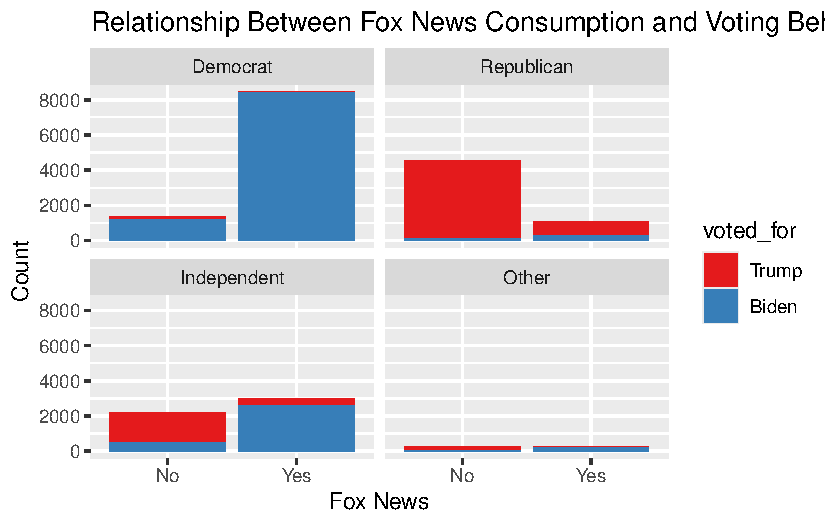
\includegraphics{paper_files/figure-pdf/unnamed-chunk-9-1.pdf}

}

\end{figure}

\begin{Shaded}
\begin{Highlighting}[]
 \CommentTok{\# scale\_color\_manual(values = c("red", "blue")) +  \# Customize colors for better visibility}
  \FunctionTok{theme\_minimal}\NormalTok{()}
\end{Highlighting}
\end{Shaded}

\begin{verbatim}
List of 136
 $ line                            :List of 6
  ..$ colour       : chr "black"
  ..$ linewidth    : num 0.5
  ..$ linetype     : num 1
  ..$ lineend      : chr "butt"
  ..$ arrow        : logi FALSE
  ..$ inherit.blank: logi TRUE
  ..- attr(*, "class")= chr [1:2] "element_line" "element"
 $ rect                            :List of 5
  ..$ fill         : chr "white"
  ..$ colour       : chr "black"
  ..$ linewidth    : num 0.5
  ..$ linetype     : num 1
  ..$ inherit.blank: logi TRUE
  ..- attr(*, "class")= chr [1:2] "element_rect" "element"
 $ text                            :List of 11
  ..$ family       : chr ""
  ..$ face         : chr "plain"
  ..$ colour       : chr "black"
  ..$ size         : num 11
  ..$ hjust        : num 0.5
  ..$ vjust        : num 0.5
  ..$ angle        : num 0
  ..$ lineheight   : num 0.9
  ..$ margin       : 'margin' num [1:4] 0points 0points 0points 0points
  .. ..- attr(*, "unit")= int 8
  ..$ debug        : logi FALSE
  ..$ inherit.blank: logi TRUE
  ..- attr(*, "class")= chr [1:2] "element_text" "element"
 $ title                           : NULL
 $ aspect.ratio                    : NULL
 $ axis.title                      : NULL
 $ axis.title.x                    :List of 11
  ..$ family       : NULL
  ..$ face         : NULL
  ..$ colour       : NULL
  ..$ size         : NULL
  ..$ hjust        : NULL
  ..$ vjust        : num 1
  ..$ angle        : NULL
  ..$ lineheight   : NULL
  ..$ margin       : 'margin' num [1:4] 2.75points 0points 0points 0points
  .. ..- attr(*, "unit")= int 8
  ..$ debug        : NULL
  ..$ inherit.blank: logi TRUE
  ..- attr(*, "class")= chr [1:2] "element_text" "element"
 $ axis.title.x.top                :List of 11
  ..$ family       : NULL
  ..$ face         : NULL
  ..$ colour       : NULL
  ..$ size         : NULL
  ..$ hjust        : NULL
  ..$ vjust        : num 0
  ..$ angle        : NULL
  ..$ lineheight   : NULL
  ..$ margin       : 'margin' num [1:4] 0points 0points 2.75points 0points
  .. ..- attr(*, "unit")= int 8
  ..$ debug        : NULL
  ..$ inherit.blank: logi TRUE
  ..- attr(*, "class")= chr [1:2] "element_text" "element"
 $ axis.title.x.bottom             : NULL
 $ axis.title.y                    :List of 11
  ..$ family       : NULL
  ..$ face         : NULL
  ..$ colour       : NULL
  ..$ size         : NULL
  ..$ hjust        : NULL
  ..$ vjust        : num 1
  ..$ angle        : num 90
  ..$ lineheight   : NULL
  ..$ margin       : 'margin' num [1:4] 0points 2.75points 0points 0points
  .. ..- attr(*, "unit")= int 8
  ..$ debug        : NULL
  ..$ inherit.blank: logi TRUE
  ..- attr(*, "class")= chr [1:2] "element_text" "element"
 $ axis.title.y.left               : NULL
 $ axis.title.y.right              :List of 11
  ..$ family       : NULL
  ..$ face         : NULL
  ..$ colour       : NULL
  ..$ size         : NULL
  ..$ hjust        : NULL
  ..$ vjust        : num 1
  ..$ angle        : num -90
  ..$ lineheight   : NULL
  ..$ margin       : 'margin' num [1:4] 0points 0points 0points 2.75points
  .. ..- attr(*, "unit")= int 8
  ..$ debug        : NULL
  ..$ inherit.blank: logi TRUE
  ..- attr(*, "class")= chr [1:2] "element_text" "element"
 $ axis.text                       :List of 11
  ..$ family       : NULL
  ..$ face         : NULL
  ..$ colour       : chr "grey30"
  ..$ size         : 'rel' num 0.8
  ..$ hjust        : NULL
  ..$ vjust        : NULL
  ..$ angle        : NULL
  ..$ lineheight   : NULL
  ..$ margin       : NULL
  ..$ debug        : NULL
  ..$ inherit.blank: logi TRUE
  ..- attr(*, "class")= chr [1:2] "element_text" "element"
 $ axis.text.x                     :List of 11
  ..$ family       : NULL
  ..$ face         : NULL
  ..$ colour       : NULL
  ..$ size         : NULL
  ..$ hjust        : NULL
  ..$ vjust        : num 1
  ..$ angle        : NULL
  ..$ lineheight   : NULL
  ..$ margin       : 'margin' num [1:4] 2.2points 0points 0points 0points
  .. ..- attr(*, "unit")= int 8
  ..$ debug        : NULL
  ..$ inherit.blank: logi TRUE
  ..- attr(*, "class")= chr [1:2] "element_text" "element"
 $ axis.text.x.top                 :List of 11
  ..$ family       : NULL
  ..$ face         : NULL
  ..$ colour       : NULL
  ..$ size         : NULL
  ..$ hjust        : NULL
  ..$ vjust        : num 0
  ..$ angle        : NULL
  ..$ lineheight   : NULL
  ..$ margin       : 'margin' num [1:4] 0points 0points 2.2points 0points
  .. ..- attr(*, "unit")= int 8
  ..$ debug        : NULL
  ..$ inherit.blank: logi TRUE
  ..- attr(*, "class")= chr [1:2] "element_text" "element"
 $ axis.text.x.bottom              : NULL
 $ axis.text.y                     :List of 11
  ..$ family       : NULL
  ..$ face         : NULL
  ..$ colour       : NULL
  ..$ size         : NULL
  ..$ hjust        : num 1
  ..$ vjust        : NULL
  ..$ angle        : NULL
  ..$ lineheight   : NULL
  ..$ margin       : 'margin' num [1:4] 0points 2.2points 0points 0points
  .. ..- attr(*, "unit")= int 8
  ..$ debug        : NULL
  ..$ inherit.blank: logi TRUE
  ..- attr(*, "class")= chr [1:2] "element_text" "element"
 $ axis.text.y.left                : NULL
 $ axis.text.y.right               :List of 11
  ..$ family       : NULL
  ..$ face         : NULL
  ..$ colour       : NULL
  ..$ size         : NULL
  ..$ hjust        : num 0
  ..$ vjust        : NULL
  ..$ angle        : NULL
  ..$ lineheight   : NULL
  ..$ margin       : 'margin' num [1:4] 0points 0points 0points 2.2points
  .. ..- attr(*, "unit")= int 8
  ..$ debug        : NULL
  ..$ inherit.blank: logi TRUE
  ..- attr(*, "class")= chr [1:2] "element_text" "element"
 $ axis.text.theta                 : NULL
 $ axis.text.r                     :List of 11
  ..$ family       : NULL
  ..$ face         : NULL
  ..$ colour       : NULL
  ..$ size         : NULL
  ..$ hjust        : num 0.5
  ..$ vjust        : NULL
  ..$ angle        : NULL
  ..$ lineheight   : NULL
  ..$ margin       : 'margin' num [1:4] 0points 2.2points 0points 2.2points
  .. ..- attr(*, "unit")= int 8
  ..$ debug        : NULL
  ..$ inherit.blank: logi TRUE
  ..- attr(*, "class")= chr [1:2] "element_text" "element"
 $ axis.ticks                      : list()
  ..- attr(*, "class")= chr [1:2] "element_blank" "element"
 $ axis.ticks.x                    : NULL
 $ axis.ticks.x.top                : NULL
 $ axis.ticks.x.bottom             : NULL
 $ axis.ticks.y                    : NULL
 $ axis.ticks.y.left               : NULL
 $ axis.ticks.y.right              : NULL
 $ axis.ticks.theta                : NULL
 $ axis.ticks.r                    : NULL
 $ axis.minor.ticks.x.top          : NULL
 $ axis.minor.ticks.x.bottom       : NULL
 $ axis.minor.ticks.y.left         : NULL
 $ axis.minor.ticks.y.right        : NULL
 $ axis.minor.ticks.theta          : NULL
 $ axis.minor.ticks.r              : NULL
 $ axis.ticks.length               : 'simpleUnit' num 2.75points
  ..- attr(*, "unit")= int 8
 $ axis.ticks.length.x             : NULL
 $ axis.ticks.length.x.top         : NULL
 $ axis.ticks.length.x.bottom      : NULL
 $ axis.ticks.length.y             : NULL
 $ axis.ticks.length.y.left        : NULL
 $ axis.ticks.length.y.right       : NULL
 $ axis.ticks.length.theta         : NULL
 $ axis.ticks.length.r             : NULL
 $ axis.minor.ticks.length         : 'rel' num 0.75
 $ axis.minor.ticks.length.x       : NULL
 $ axis.minor.ticks.length.x.top   : NULL
 $ axis.minor.ticks.length.x.bottom: NULL
 $ axis.minor.ticks.length.y       : NULL
 $ axis.minor.ticks.length.y.left  : NULL
 $ axis.minor.ticks.length.y.right : NULL
 $ axis.minor.ticks.length.theta   : NULL
 $ axis.minor.ticks.length.r       : NULL
 $ axis.line                       : list()
  ..- attr(*, "class")= chr [1:2] "element_blank" "element"
 $ axis.line.x                     : NULL
 $ axis.line.x.top                 : NULL
 $ axis.line.x.bottom              : NULL
 $ axis.line.y                     : NULL
 $ axis.line.y.left                : NULL
 $ axis.line.y.right               : NULL
 $ axis.line.theta                 : NULL
 $ axis.line.r                     : NULL
 $ legend.background               : list()
  ..- attr(*, "class")= chr [1:2] "element_blank" "element"
 $ legend.margin                   : 'margin' num [1:4] 5.5points 5.5points 5.5points 5.5points
  ..- attr(*, "unit")= int 8
 $ legend.spacing                  : 'simpleUnit' num 11points
  ..- attr(*, "unit")= int 8
 $ legend.spacing.x                : NULL
 $ legend.spacing.y                : NULL
 $ legend.key                      : list()
  ..- attr(*, "class")= chr [1:2] "element_blank" "element"
 $ legend.key.size                 : 'simpleUnit' num 1.2lines
  ..- attr(*, "unit")= int 3
 $ legend.key.height               : NULL
 $ legend.key.width                : NULL
 $ legend.key.spacing              : 'simpleUnit' num 5.5points
  ..- attr(*, "unit")= int 8
 $ legend.key.spacing.x            : NULL
 $ legend.key.spacing.y            : NULL
 $ legend.frame                    : NULL
 $ legend.ticks                    : NULL
 $ legend.ticks.length             : 'rel' num 0.2
 $ legend.axis.line                : NULL
 $ legend.text                     :List of 11
  ..$ family       : NULL
  ..$ face         : NULL
  ..$ colour       : NULL
  ..$ size         : 'rel' num 0.8
  ..$ hjust        : NULL
  ..$ vjust        : NULL
  ..$ angle        : NULL
  ..$ lineheight   : NULL
  ..$ margin       : NULL
  ..$ debug        : NULL
  ..$ inherit.blank: logi TRUE
  ..- attr(*, "class")= chr [1:2] "element_text" "element"
 $ legend.text.position            : NULL
 $ legend.title                    :List of 11
  ..$ family       : NULL
  ..$ face         : NULL
  ..$ colour       : NULL
  ..$ size         : NULL
  ..$ hjust        : num 0
  ..$ vjust        : NULL
  ..$ angle        : NULL
  ..$ lineheight   : NULL
  ..$ margin       : NULL
  ..$ debug        : NULL
  ..$ inherit.blank: logi TRUE
  ..- attr(*, "class")= chr [1:2] "element_text" "element"
 $ legend.title.position           : NULL
 $ legend.position                 : chr "right"
 $ legend.position.inside          : NULL
 $ legend.direction                : NULL
 $ legend.byrow                    : NULL
 $ legend.justification            : chr "center"
 $ legend.justification.top        : NULL
 $ legend.justification.bottom     : NULL
 $ legend.justification.left       : NULL
 $ legend.justification.right      : NULL
 $ legend.justification.inside     : NULL
 $ legend.location                 : NULL
 $ legend.box                      : NULL
 $ legend.box.just                 : NULL
 $ legend.box.margin               : 'margin' num [1:4] 0cm 0cm 0cm 0cm
  ..- attr(*, "unit")= int 1
 $ legend.box.background           : list()
  ..- attr(*, "class")= chr [1:2] "element_blank" "element"
 $ legend.box.spacing              : 'simpleUnit' num 11points
  ..- attr(*, "unit")= int 8
  [list output truncated]
 - attr(*, "class")= chr [1:2] "theme" "gg"
 - attr(*, "complete")= logi TRUE
 - attr(*, "validate")= logi TRUE
\end{verbatim}

\begin{Shaded}
\begin{Highlighting}[]
\CommentTok{\# Change labels for Fox\_News variable}
\NormalTok{ces2020}\SpecialCharTok{$}\NormalTok{CNN }\OtherTok{\textless{}{-}} \FunctionTok{factor}\NormalTok{(ces2020}\SpecialCharTok{$}\NormalTok{CNN, }\AttributeTok{labels =} \FunctionTok{c}\NormalTok{(}\StringTok{"No"}\NormalTok{, }\StringTok{"Yes"}\NormalTok{))}

\FunctionTok{ggplot}\NormalTok{(ces2020, }\FunctionTok{aes}\NormalTok{(}\AttributeTok{x =}\NormalTok{ CNN, }\AttributeTok{fill =}\NormalTok{ voted\_for)) }\SpecialCharTok{+}
  \FunctionTok{geom\_bar}\NormalTok{() }\SpecialCharTok{+}
  \FunctionTok{facet\_wrap}\NormalTok{(}\AttributeTok{facets =} \FunctionTok{vars}\NormalTok{(Party)) }\SpecialCharTok{+}
  \FunctionTok{labs}\NormalTok{(}\AttributeTok{title =} \StringTok{"Relationship Between CNN Consumption and Voting Behavior"}\NormalTok{,}
       \AttributeTok{x =} \StringTok{"CNN"}\NormalTok{,}
       \AttributeTok{y =} \StringTok{"Count"}\NormalTok{,}
       \AttributeTok{color =} \StringTok{"Voted for Biden (1) or Trump (0)"}\NormalTok{) }\SpecialCharTok{+}
  \FunctionTok{scale\_fill\_brewer}\NormalTok{(}\AttributeTok{palette =} \StringTok{"Set1"}\NormalTok{)}
\end{Highlighting}
\end{Shaded}

\begin{figure}[H]

{\centering 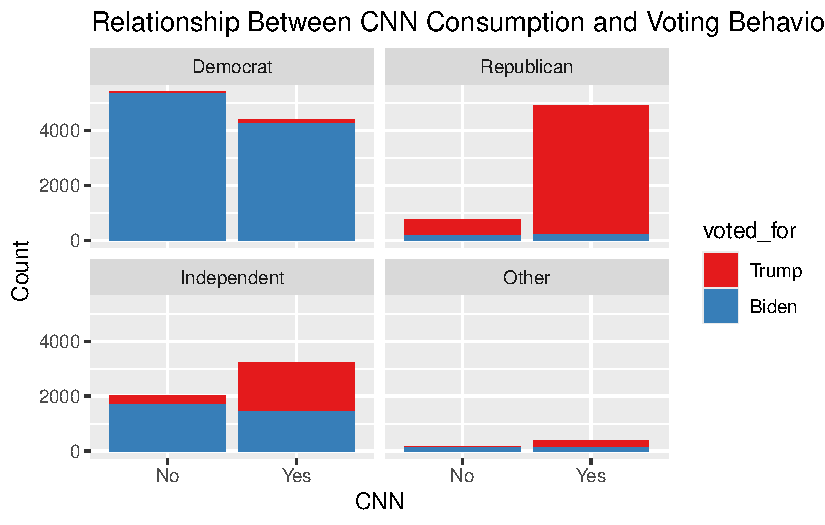
\includegraphics{paper_files/figure-pdf/unnamed-chunk-10-1.pdf}

}

\end{figure}

\begin{Shaded}
\begin{Highlighting}[]
 \CommentTok{\# scale\_color\_manual(values = c("red", "blue")) +  \# Customize colors for better visibility}
  \FunctionTok{theme\_minimal}\NormalTok{()}
\end{Highlighting}
\end{Shaded}

\begin{verbatim}
List of 136
 $ line                            :List of 6
  ..$ colour       : chr "black"
  ..$ linewidth    : num 0.5
  ..$ linetype     : num 1
  ..$ lineend      : chr "butt"
  ..$ arrow        : logi FALSE
  ..$ inherit.blank: logi TRUE
  ..- attr(*, "class")= chr [1:2] "element_line" "element"
 $ rect                            :List of 5
  ..$ fill         : chr "white"
  ..$ colour       : chr "black"
  ..$ linewidth    : num 0.5
  ..$ linetype     : num 1
  ..$ inherit.blank: logi TRUE
  ..- attr(*, "class")= chr [1:2] "element_rect" "element"
 $ text                            :List of 11
  ..$ family       : chr ""
  ..$ face         : chr "plain"
  ..$ colour       : chr "black"
  ..$ size         : num 11
  ..$ hjust        : num 0.5
  ..$ vjust        : num 0.5
  ..$ angle        : num 0
  ..$ lineheight   : num 0.9
  ..$ margin       : 'margin' num [1:4] 0points 0points 0points 0points
  .. ..- attr(*, "unit")= int 8
  ..$ debug        : logi FALSE
  ..$ inherit.blank: logi TRUE
  ..- attr(*, "class")= chr [1:2] "element_text" "element"
 $ title                           : NULL
 $ aspect.ratio                    : NULL
 $ axis.title                      : NULL
 $ axis.title.x                    :List of 11
  ..$ family       : NULL
  ..$ face         : NULL
  ..$ colour       : NULL
  ..$ size         : NULL
  ..$ hjust        : NULL
  ..$ vjust        : num 1
  ..$ angle        : NULL
  ..$ lineheight   : NULL
  ..$ margin       : 'margin' num [1:4] 2.75points 0points 0points 0points
  .. ..- attr(*, "unit")= int 8
  ..$ debug        : NULL
  ..$ inherit.blank: logi TRUE
  ..- attr(*, "class")= chr [1:2] "element_text" "element"
 $ axis.title.x.top                :List of 11
  ..$ family       : NULL
  ..$ face         : NULL
  ..$ colour       : NULL
  ..$ size         : NULL
  ..$ hjust        : NULL
  ..$ vjust        : num 0
  ..$ angle        : NULL
  ..$ lineheight   : NULL
  ..$ margin       : 'margin' num [1:4] 0points 0points 2.75points 0points
  .. ..- attr(*, "unit")= int 8
  ..$ debug        : NULL
  ..$ inherit.blank: logi TRUE
  ..- attr(*, "class")= chr [1:2] "element_text" "element"
 $ axis.title.x.bottom             : NULL
 $ axis.title.y                    :List of 11
  ..$ family       : NULL
  ..$ face         : NULL
  ..$ colour       : NULL
  ..$ size         : NULL
  ..$ hjust        : NULL
  ..$ vjust        : num 1
  ..$ angle        : num 90
  ..$ lineheight   : NULL
  ..$ margin       : 'margin' num [1:4] 0points 2.75points 0points 0points
  .. ..- attr(*, "unit")= int 8
  ..$ debug        : NULL
  ..$ inherit.blank: logi TRUE
  ..- attr(*, "class")= chr [1:2] "element_text" "element"
 $ axis.title.y.left               : NULL
 $ axis.title.y.right              :List of 11
  ..$ family       : NULL
  ..$ face         : NULL
  ..$ colour       : NULL
  ..$ size         : NULL
  ..$ hjust        : NULL
  ..$ vjust        : num 1
  ..$ angle        : num -90
  ..$ lineheight   : NULL
  ..$ margin       : 'margin' num [1:4] 0points 0points 0points 2.75points
  .. ..- attr(*, "unit")= int 8
  ..$ debug        : NULL
  ..$ inherit.blank: logi TRUE
  ..- attr(*, "class")= chr [1:2] "element_text" "element"
 $ axis.text                       :List of 11
  ..$ family       : NULL
  ..$ face         : NULL
  ..$ colour       : chr "grey30"
  ..$ size         : 'rel' num 0.8
  ..$ hjust        : NULL
  ..$ vjust        : NULL
  ..$ angle        : NULL
  ..$ lineheight   : NULL
  ..$ margin       : NULL
  ..$ debug        : NULL
  ..$ inherit.blank: logi TRUE
  ..- attr(*, "class")= chr [1:2] "element_text" "element"
 $ axis.text.x                     :List of 11
  ..$ family       : NULL
  ..$ face         : NULL
  ..$ colour       : NULL
  ..$ size         : NULL
  ..$ hjust        : NULL
  ..$ vjust        : num 1
  ..$ angle        : NULL
  ..$ lineheight   : NULL
  ..$ margin       : 'margin' num [1:4] 2.2points 0points 0points 0points
  .. ..- attr(*, "unit")= int 8
  ..$ debug        : NULL
  ..$ inherit.blank: logi TRUE
  ..- attr(*, "class")= chr [1:2] "element_text" "element"
 $ axis.text.x.top                 :List of 11
  ..$ family       : NULL
  ..$ face         : NULL
  ..$ colour       : NULL
  ..$ size         : NULL
  ..$ hjust        : NULL
  ..$ vjust        : num 0
  ..$ angle        : NULL
  ..$ lineheight   : NULL
  ..$ margin       : 'margin' num [1:4] 0points 0points 2.2points 0points
  .. ..- attr(*, "unit")= int 8
  ..$ debug        : NULL
  ..$ inherit.blank: logi TRUE
  ..- attr(*, "class")= chr [1:2] "element_text" "element"
 $ axis.text.x.bottom              : NULL
 $ axis.text.y                     :List of 11
  ..$ family       : NULL
  ..$ face         : NULL
  ..$ colour       : NULL
  ..$ size         : NULL
  ..$ hjust        : num 1
  ..$ vjust        : NULL
  ..$ angle        : NULL
  ..$ lineheight   : NULL
  ..$ margin       : 'margin' num [1:4] 0points 2.2points 0points 0points
  .. ..- attr(*, "unit")= int 8
  ..$ debug        : NULL
  ..$ inherit.blank: logi TRUE
  ..- attr(*, "class")= chr [1:2] "element_text" "element"
 $ axis.text.y.left                : NULL
 $ axis.text.y.right               :List of 11
  ..$ family       : NULL
  ..$ face         : NULL
  ..$ colour       : NULL
  ..$ size         : NULL
  ..$ hjust        : num 0
  ..$ vjust        : NULL
  ..$ angle        : NULL
  ..$ lineheight   : NULL
  ..$ margin       : 'margin' num [1:4] 0points 0points 0points 2.2points
  .. ..- attr(*, "unit")= int 8
  ..$ debug        : NULL
  ..$ inherit.blank: logi TRUE
  ..- attr(*, "class")= chr [1:2] "element_text" "element"
 $ axis.text.theta                 : NULL
 $ axis.text.r                     :List of 11
  ..$ family       : NULL
  ..$ face         : NULL
  ..$ colour       : NULL
  ..$ size         : NULL
  ..$ hjust        : num 0.5
  ..$ vjust        : NULL
  ..$ angle        : NULL
  ..$ lineheight   : NULL
  ..$ margin       : 'margin' num [1:4] 0points 2.2points 0points 2.2points
  .. ..- attr(*, "unit")= int 8
  ..$ debug        : NULL
  ..$ inherit.blank: logi TRUE
  ..- attr(*, "class")= chr [1:2] "element_text" "element"
 $ axis.ticks                      : list()
  ..- attr(*, "class")= chr [1:2] "element_blank" "element"
 $ axis.ticks.x                    : NULL
 $ axis.ticks.x.top                : NULL
 $ axis.ticks.x.bottom             : NULL
 $ axis.ticks.y                    : NULL
 $ axis.ticks.y.left               : NULL
 $ axis.ticks.y.right              : NULL
 $ axis.ticks.theta                : NULL
 $ axis.ticks.r                    : NULL
 $ axis.minor.ticks.x.top          : NULL
 $ axis.minor.ticks.x.bottom       : NULL
 $ axis.minor.ticks.y.left         : NULL
 $ axis.minor.ticks.y.right        : NULL
 $ axis.minor.ticks.theta          : NULL
 $ axis.minor.ticks.r              : NULL
 $ axis.ticks.length               : 'simpleUnit' num 2.75points
  ..- attr(*, "unit")= int 8
 $ axis.ticks.length.x             : NULL
 $ axis.ticks.length.x.top         : NULL
 $ axis.ticks.length.x.bottom      : NULL
 $ axis.ticks.length.y             : NULL
 $ axis.ticks.length.y.left        : NULL
 $ axis.ticks.length.y.right       : NULL
 $ axis.ticks.length.theta         : NULL
 $ axis.ticks.length.r             : NULL
 $ axis.minor.ticks.length         : 'rel' num 0.75
 $ axis.minor.ticks.length.x       : NULL
 $ axis.minor.ticks.length.x.top   : NULL
 $ axis.minor.ticks.length.x.bottom: NULL
 $ axis.minor.ticks.length.y       : NULL
 $ axis.minor.ticks.length.y.left  : NULL
 $ axis.minor.ticks.length.y.right : NULL
 $ axis.minor.ticks.length.theta   : NULL
 $ axis.minor.ticks.length.r       : NULL
 $ axis.line                       : list()
  ..- attr(*, "class")= chr [1:2] "element_blank" "element"
 $ axis.line.x                     : NULL
 $ axis.line.x.top                 : NULL
 $ axis.line.x.bottom              : NULL
 $ axis.line.y                     : NULL
 $ axis.line.y.left                : NULL
 $ axis.line.y.right               : NULL
 $ axis.line.theta                 : NULL
 $ axis.line.r                     : NULL
 $ legend.background               : list()
  ..- attr(*, "class")= chr [1:2] "element_blank" "element"
 $ legend.margin                   : 'margin' num [1:4] 5.5points 5.5points 5.5points 5.5points
  ..- attr(*, "unit")= int 8
 $ legend.spacing                  : 'simpleUnit' num 11points
  ..- attr(*, "unit")= int 8
 $ legend.spacing.x                : NULL
 $ legend.spacing.y                : NULL
 $ legend.key                      : list()
  ..- attr(*, "class")= chr [1:2] "element_blank" "element"
 $ legend.key.size                 : 'simpleUnit' num 1.2lines
  ..- attr(*, "unit")= int 3
 $ legend.key.height               : NULL
 $ legend.key.width                : NULL
 $ legend.key.spacing              : 'simpleUnit' num 5.5points
  ..- attr(*, "unit")= int 8
 $ legend.key.spacing.x            : NULL
 $ legend.key.spacing.y            : NULL
 $ legend.frame                    : NULL
 $ legend.ticks                    : NULL
 $ legend.ticks.length             : 'rel' num 0.2
 $ legend.axis.line                : NULL
 $ legend.text                     :List of 11
  ..$ family       : NULL
  ..$ face         : NULL
  ..$ colour       : NULL
  ..$ size         : 'rel' num 0.8
  ..$ hjust        : NULL
  ..$ vjust        : NULL
  ..$ angle        : NULL
  ..$ lineheight   : NULL
  ..$ margin       : NULL
  ..$ debug        : NULL
  ..$ inherit.blank: logi TRUE
  ..- attr(*, "class")= chr [1:2] "element_text" "element"
 $ legend.text.position            : NULL
 $ legend.title                    :List of 11
  ..$ family       : NULL
  ..$ face         : NULL
  ..$ colour       : NULL
  ..$ size         : NULL
  ..$ hjust        : num 0
  ..$ vjust        : NULL
  ..$ angle        : NULL
  ..$ lineheight   : NULL
  ..$ margin       : NULL
  ..$ debug        : NULL
  ..$ inherit.blank: logi TRUE
  ..- attr(*, "class")= chr [1:2] "element_text" "element"
 $ legend.title.position           : NULL
 $ legend.position                 : chr "right"
 $ legend.position.inside          : NULL
 $ legend.direction                : NULL
 $ legend.byrow                    : NULL
 $ legend.justification            : chr "center"
 $ legend.justification.top        : NULL
 $ legend.justification.bottom     : NULL
 $ legend.justification.left       : NULL
 $ legend.justification.right      : NULL
 $ legend.justification.inside     : NULL
 $ legend.location                 : NULL
 $ legend.box                      : NULL
 $ legend.box.just                 : NULL
 $ legend.box.margin               : 'margin' num [1:4] 0cm 0cm 0cm 0cm
  ..- attr(*, "unit")= int 1
 $ legend.box.background           : list()
  ..- attr(*, "class")= chr [1:2] "element_blank" "element"
 $ legend.box.spacing              : 'simpleUnit' num 11points
  ..- attr(*, "unit")= int 8
  [list output truncated]
 - attr(*, "class")= chr [1:2] "theme" "gg"
 - attr(*, "complete")= logi TRUE
 - attr(*, "validate")= logi TRUE
\end{verbatim}

\begin{Shaded}
\begin{Highlighting}[]
\NormalTok{ces2020}\SpecialCharTok{$}\NormalTok{TV\_type }\OtherTok{\textless{}{-}} \FunctionTok{factor}\NormalTok{(ces2020}\SpecialCharTok{$}\NormalTok{TV\_type, }\AttributeTok{labels =} \FunctionTok{c}\NormalTok{(}\StringTok{"National \& Local"}\NormalTok{, }\StringTok{"National"}\NormalTok{))}

\NormalTok{scatter\_plot }\OtherTok{\textless{}{-}} \FunctionTok{ggplot}\NormalTok{(ces2020, }\FunctionTok{aes}\NormalTok{(}\AttributeTok{x =}\NormalTok{ TV\_type, }\AttributeTok{fill =}\NormalTok{ voted\_for)) }\SpecialCharTok{+}
  \FunctionTok{geom\_bar}\NormalTok{() }\SpecialCharTok{+}
  \FunctionTok{facet\_wrap}\NormalTok{(}\AttributeTok{facets =} \FunctionTok{vars}\NormalTok{(Party)) }\SpecialCharTok{+}
  \FunctionTok{labs}\NormalTok{(}\AttributeTok{title =} \StringTok{"Relationship Between TV News Consumption and Voting Behavior"}\NormalTok{,}
       \AttributeTok{x =} \StringTok{"TV Type"}\NormalTok{,}
       \AttributeTok{y =} \StringTok{"Count"}\NormalTok{,}
       \AttributeTok{color =} \StringTok{"Voted for Biden (1) or Trump (0)"}\NormalTok{) }\SpecialCharTok{+}
  \FunctionTok{scale\_fill\_brewer}\NormalTok{(}\AttributeTok{palette =} \StringTok{"Set1"}\NormalTok{)}
 \CommentTok{\# scale\_color\_manual(values = c("red", "blue")) +  \# Customize colors for better visibility}
  \FunctionTok{theme\_minimal}\NormalTok{()}
\end{Highlighting}
\end{Shaded}

\begin{verbatim}
List of 136
 $ line                            :List of 6
  ..$ colour       : chr "black"
  ..$ linewidth    : num 0.5
  ..$ linetype     : num 1
  ..$ lineend      : chr "butt"
  ..$ arrow        : logi FALSE
  ..$ inherit.blank: logi TRUE
  ..- attr(*, "class")= chr [1:2] "element_line" "element"
 $ rect                            :List of 5
  ..$ fill         : chr "white"
  ..$ colour       : chr "black"
  ..$ linewidth    : num 0.5
  ..$ linetype     : num 1
  ..$ inherit.blank: logi TRUE
  ..- attr(*, "class")= chr [1:2] "element_rect" "element"
 $ text                            :List of 11
  ..$ family       : chr ""
  ..$ face         : chr "plain"
  ..$ colour       : chr "black"
  ..$ size         : num 11
  ..$ hjust        : num 0.5
  ..$ vjust        : num 0.5
  ..$ angle        : num 0
  ..$ lineheight   : num 0.9
  ..$ margin       : 'margin' num [1:4] 0points 0points 0points 0points
  .. ..- attr(*, "unit")= int 8
  ..$ debug        : logi FALSE
  ..$ inherit.blank: logi TRUE
  ..- attr(*, "class")= chr [1:2] "element_text" "element"
 $ title                           : NULL
 $ aspect.ratio                    : NULL
 $ axis.title                      : NULL
 $ axis.title.x                    :List of 11
  ..$ family       : NULL
  ..$ face         : NULL
  ..$ colour       : NULL
  ..$ size         : NULL
  ..$ hjust        : NULL
  ..$ vjust        : num 1
  ..$ angle        : NULL
  ..$ lineheight   : NULL
  ..$ margin       : 'margin' num [1:4] 2.75points 0points 0points 0points
  .. ..- attr(*, "unit")= int 8
  ..$ debug        : NULL
  ..$ inherit.blank: logi TRUE
  ..- attr(*, "class")= chr [1:2] "element_text" "element"
 $ axis.title.x.top                :List of 11
  ..$ family       : NULL
  ..$ face         : NULL
  ..$ colour       : NULL
  ..$ size         : NULL
  ..$ hjust        : NULL
  ..$ vjust        : num 0
  ..$ angle        : NULL
  ..$ lineheight   : NULL
  ..$ margin       : 'margin' num [1:4] 0points 0points 2.75points 0points
  .. ..- attr(*, "unit")= int 8
  ..$ debug        : NULL
  ..$ inherit.blank: logi TRUE
  ..- attr(*, "class")= chr [1:2] "element_text" "element"
 $ axis.title.x.bottom             : NULL
 $ axis.title.y                    :List of 11
  ..$ family       : NULL
  ..$ face         : NULL
  ..$ colour       : NULL
  ..$ size         : NULL
  ..$ hjust        : NULL
  ..$ vjust        : num 1
  ..$ angle        : num 90
  ..$ lineheight   : NULL
  ..$ margin       : 'margin' num [1:4] 0points 2.75points 0points 0points
  .. ..- attr(*, "unit")= int 8
  ..$ debug        : NULL
  ..$ inherit.blank: logi TRUE
  ..- attr(*, "class")= chr [1:2] "element_text" "element"
 $ axis.title.y.left               : NULL
 $ axis.title.y.right              :List of 11
  ..$ family       : NULL
  ..$ face         : NULL
  ..$ colour       : NULL
  ..$ size         : NULL
  ..$ hjust        : NULL
  ..$ vjust        : num 1
  ..$ angle        : num -90
  ..$ lineheight   : NULL
  ..$ margin       : 'margin' num [1:4] 0points 0points 0points 2.75points
  .. ..- attr(*, "unit")= int 8
  ..$ debug        : NULL
  ..$ inherit.blank: logi TRUE
  ..- attr(*, "class")= chr [1:2] "element_text" "element"
 $ axis.text                       :List of 11
  ..$ family       : NULL
  ..$ face         : NULL
  ..$ colour       : chr "grey30"
  ..$ size         : 'rel' num 0.8
  ..$ hjust        : NULL
  ..$ vjust        : NULL
  ..$ angle        : NULL
  ..$ lineheight   : NULL
  ..$ margin       : NULL
  ..$ debug        : NULL
  ..$ inherit.blank: logi TRUE
  ..- attr(*, "class")= chr [1:2] "element_text" "element"
 $ axis.text.x                     :List of 11
  ..$ family       : NULL
  ..$ face         : NULL
  ..$ colour       : NULL
  ..$ size         : NULL
  ..$ hjust        : NULL
  ..$ vjust        : num 1
  ..$ angle        : NULL
  ..$ lineheight   : NULL
  ..$ margin       : 'margin' num [1:4] 2.2points 0points 0points 0points
  .. ..- attr(*, "unit")= int 8
  ..$ debug        : NULL
  ..$ inherit.blank: logi TRUE
  ..- attr(*, "class")= chr [1:2] "element_text" "element"
 $ axis.text.x.top                 :List of 11
  ..$ family       : NULL
  ..$ face         : NULL
  ..$ colour       : NULL
  ..$ size         : NULL
  ..$ hjust        : NULL
  ..$ vjust        : num 0
  ..$ angle        : NULL
  ..$ lineheight   : NULL
  ..$ margin       : 'margin' num [1:4] 0points 0points 2.2points 0points
  .. ..- attr(*, "unit")= int 8
  ..$ debug        : NULL
  ..$ inherit.blank: logi TRUE
  ..- attr(*, "class")= chr [1:2] "element_text" "element"
 $ axis.text.x.bottom              : NULL
 $ axis.text.y                     :List of 11
  ..$ family       : NULL
  ..$ face         : NULL
  ..$ colour       : NULL
  ..$ size         : NULL
  ..$ hjust        : num 1
  ..$ vjust        : NULL
  ..$ angle        : NULL
  ..$ lineheight   : NULL
  ..$ margin       : 'margin' num [1:4] 0points 2.2points 0points 0points
  .. ..- attr(*, "unit")= int 8
  ..$ debug        : NULL
  ..$ inherit.blank: logi TRUE
  ..- attr(*, "class")= chr [1:2] "element_text" "element"
 $ axis.text.y.left                : NULL
 $ axis.text.y.right               :List of 11
  ..$ family       : NULL
  ..$ face         : NULL
  ..$ colour       : NULL
  ..$ size         : NULL
  ..$ hjust        : num 0
  ..$ vjust        : NULL
  ..$ angle        : NULL
  ..$ lineheight   : NULL
  ..$ margin       : 'margin' num [1:4] 0points 0points 0points 2.2points
  .. ..- attr(*, "unit")= int 8
  ..$ debug        : NULL
  ..$ inherit.blank: logi TRUE
  ..- attr(*, "class")= chr [1:2] "element_text" "element"
 $ axis.text.theta                 : NULL
 $ axis.text.r                     :List of 11
  ..$ family       : NULL
  ..$ face         : NULL
  ..$ colour       : NULL
  ..$ size         : NULL
  ..$ hjust        : num 0.5
  ..$ vjust        : NULL
  ..$ angle        : NULL
  ..$ lineheight   : NULL
  ..$ margin       : 'margin' num [1:4] 0points 2.2points 0points 2.2points
  .. ..- attr(*, "unit")= int 8
  ..$ debug        : NULL
  ..$ inherit.blank: logi TRUE
  ..- attr(*, "class")= chr [1:2] "element_text" "element"
 $ axis.ticks                      : list()
  ..- attr(*, "class")= chr [1:2] "element_blank" "element"
 $ axis.ticks.x                    : NULL
 $ axis.ticks.x.top                : NULL
 $ axis.ticks.x.bottom             : NULL
 $ axis.ticks.y                    : NULL
 $ axis.ticks.y.left               : NULL
 $ axis.ticks.y.right              : NULL
 $ axis.ticks.theta                : NULL
 $ axis.ticks.r                    : NULL
 $ axis.minor.ticks.x.top          : NULL
 $ axis.minor.ticks.x.bottom       : NULL
 $ axis.minor.ticks.y.left         : NULL
 $ axis.minor.ticks.y.right        : NULL
 $ axis.minor.ticks.theta          : NULL
 $ axis.minor.ticks.r              : NULL
 $ axis.ticks.length               : 'simpleUnit' num 2.75points
  ..- attr(*, "unit")= int 8
 $ axis.ticks.length.x             : NULL
 $ axis.ticks.length.x.top         : NULL
 $ axis.ticks.length.x.bottom      : NULL
 $ axis.ticks.length.y             : NULL
 $ axis.ticks.length.y.left        : NULL
 $ axis.ticks.length.y.right       : NULL
 $ axis.ticks.length.theta         : NULL
 $ axis.ticks.length.r             : NULL
 $ axis.minor.ticks.length         : 'rel' num 0.75
 $ axis.minor.ticks.length.x       : NULL
 $ axis.minor.ticks.length.x.top   : NULL
 $ axis.minor.ticks.length.x.bottom: NULL
 $ axis.minor.ticks.length.y       : NULL
 $ axis.minor.ticks.length.y.left  : NULL
 $ axis.minor.ticks.length.y.right : NULL
 $ axis.minor.ticks.length.theta   : NULL
 $ axis.minor.ticks.length.r       : NULL
 $ axis.line                       : list()
  ..- attr(*, "class")= chr [1:2] "element_blank" "element"
 $ axis.line.x                     : NULL
 $ axis.line.x.top                 : NULL
 $ axis.line.x.bottom              : NULL
 $ axis.line.y                     : NULL
 $ axis.line.y.left                : NULL
 $ axis.line.y.right               : NULL
 $ axis.line.theta                 : NULL
 $ axis.line.r                     : NULL
 $ legend.background               : list()
  ..- attr(*, "class")= chr [1:2] "element_blank" "element"
 $ legend.margin                   : 'margin' num [1:4] 5.5points 5.5points 5.5points 5.5points
  ..- attr(*, "unit")= int 8
 $ legend.spacing                  : 'simpleUnit' num 11points
  ..- attr(*, "unit")= int 8
 $ legend.spacing.x                : NULL
 $ legend.spacing.y                : NULL
 $ legend.key                      : list()
  ..- attr(*, "class")= chr [1:2] "element_blank" "element"
 $ legend.key.size                 : 'simpleUnit' num 1.2lines
  ..- attr(*, "unit")= int 3
 $ legend.key.height               : NULL
 $ legend.key.width                : NULL
 $ legend.key.spacing              : 'simpleUnit' num 5.5points
  ..- attr(*, "unit")= int 8
 $ legend.key.spacing.x            : NULL
 $ legend.key.spacing.y            : NULL
 $ legend.frame                    : NULL
 $ legend.ticks                    : NULL
 $ legend.ticks.length             : 'rel' num 0.2
 $ legend.axis.line                : NULL
 $ legend.text                     :List of 11
  ..$ family       : NULL
  ..$ face         : NULL
  ..$ colour       : NULL
  ..$ size         : 'rel' num 0.8
  ..$ hjust        : NULL
  ..$ vjust        : NULL
  ..$ angle        : NULL
  ..$ lineheight   : NULL
  ..$ margin       : NULL
  ..$ debug        : NULL
  ..$ inherit.blank: logi TRUE
  ..- attr(*, "class")= chr [1:2] "element_text" "element"
 $ legend.text.position            : NULL
 $ legend.title                    :List of 11
  ..$ family       : NULL
  ..$ face         : NULL
  ..$ colour       : NULL
  ..$ size         : NULL
  ..$ hjust        : num 0
  ..$ vjust        : NULL
  ..$ angle        : NULL
  ..$ lineheight   : NULL
  ..$ margin       : NULL
  ..$ debug        : NULL
  ..$ inherit.blank: logi TRUE
  ..- attr(*, "class")= chr [1:2] "element_text" "element"
 $ legend.title.position           : NULL
 $ legend.position                 : chr "right"
 $ legend.position.inside          : NULL
 $ legend.direction                : NULL
 $ legend.byrow                    : NULL
 $ legend.justification            : chr "center"
 $ legend.justification.top        : NULL
 $ legend.justification.bottom     : NULL
 $ legend.justification.left       : NULL
 $ legend.justification.right      : NULL
 $ legend.justification.inside     : NULL
 $ legend.location                 : NULL
 $ legend.box                      : NULL
 $ legend.box.just                 : NULL
 $ legend.box.margin               : 'margin' num [1:4] 0cm 0cm 0cm 0cm
  ..- attr(*, "unit")= int 1
 $ legend.box.background           : list()
  ..- attr(*, "class")= chr [1:2] "element_blank" "element"
 $ legend.box.spacing              : 'simpleUnit' num 11points
  ..- attr(*, "unit")= int 8
  [list output truncated]
 - attr(*, "class")= chr [1:2] "theme" "gg"
 - attr(*, "complete")= logi TRUE
 - attr(*, "validate")= logi TRUE
\end{verbatim}

\begin{Shaded}
\begin{Highlighting}[]
\CommentTok{\# Show the plot}
\NormalTok{scatter\_plot}
\end{Highlighting}
\end{Shaded}

\begin{figure}[H]

{\centering 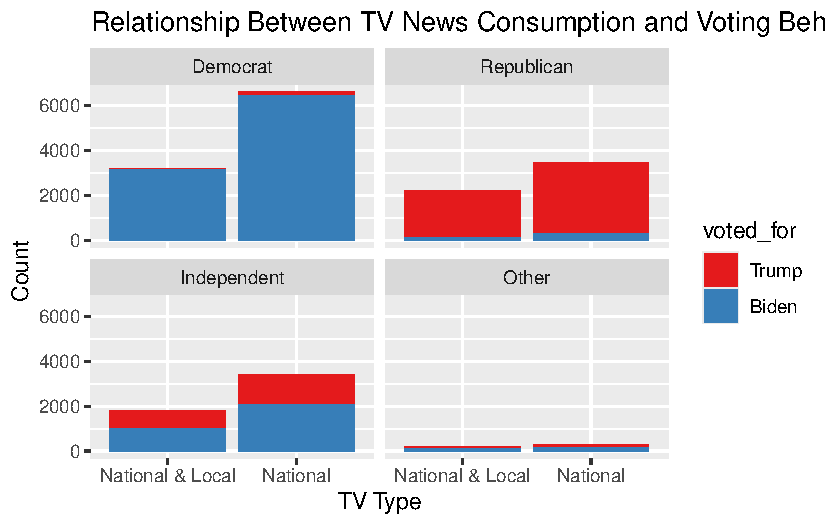
\includegraphics{paper_files/figure-pdf/unnamed-chunk-11-1.pdf}

}

\end{figure}

Our results are summarized in Table~\ref{tbl-modelresults}.

\hypertarget{tbl-modelresults}{}
\begin{table}
\caption{\label{tbl-modelresults}Explanatory models of flight time based on wing width and wing length }\tabularnewline

\centering
\begin{tabular}[t]{lc}
\toprule
  & Support Biden\\
\midrule
(Intercept) & \num{3.630}\\
 & (\num{0.307})\\
ABCYes & \num{0.468}\\
 & (\num{0.189})\\
CBSYes & \num{0.123}\\
 & \vphantom{1} (\num{0.209})\\
NBCYes & \num{0.056}\\
 & (\num{0.192})\\
CNNYes & \num{1.631}\\
 & (\num{0.209})\\
Fox\_NewsYes & \num{-3.128}\\
 & (\num{0.202})\\
MSNBCYes & \num{1.457}\\
 & (\num{0.242})\\
PBSYes & \num{0.681}\\
 & (\num{0.284})\\
OtherYes & \num{-1.218}\\
 & (\num{0.275})\\
TV\_typeNational Newscast & \num{-0.024}\\
 & (\num{0.218})\\
PartyIndependent & \num{-2.799}\\
 & (\num{0.267})\\
PartyOther & \num{-2.429}\\
 & (\num{0.465})\\
PartyRepublican & \num{-5.484}\\
 & (\num{0.306})\\
\midrule
Num.Obs. & \num{2500}\\
R2 & \num{0.786}\\
Log.Lik. & \num{-429.645}\\
ELPD & \num{-443.1}\\
ELPD s.e. & \num{26.9}\\
LOOIC & \num{886.1}\\
LOOIC s.e. & \num{53.8}\\
WAIC & \num{886.1}\\
RMSE & \num{0.22}\\
\bottomrule
\end{tabular}
\end{table}

\begin{Shaded}
\begin{Highlighting}[]
\CommentTok{\# Load necessary libraries}
\FunctionTok{library}\NormalTok{(car)}
\end{Highlighting}
\end{Shaded}

\begin{verbatim}
Loading required package: carData
\end{verbatim}

\begin{verbatim}

Attaching package: 'car'
\end{verbatim}

\begin{verbatim}
The following object is masked from 'package:rstanarm':

    logit
\end{verbatim}

\begin{verbatim}
The following object is masked from 'package:dplyr':

    recode
\end{verbatim}

\begin{verbatim}
The following object is masked from 'package:purrr':

    some
\end{verbatim}

\begin{Shaded}
\begin{Highlighting}[]
\CommentTok{\# Check for multicollinearity using VIF}
\FunctionTok{vif}\NormalTok{(political\_preferences)}
\end{Highlighting}
\end{Shaded}

\begin{verbatim}
             GVIF Df GVIF^(1/(2*Df))
ABC      1.135455  1        1.065577
CBS      1.213237  1        1.101471
NBC      1.104373  1        1.050891
CNN      1.185597  1        1.088851
Fox_News 1.223857  1        1.106281
MSNBC    1.151721  1        1.073183
PBS      1.069843  1        1.034332
Other    1.053979  1        1.026635
TV_type  1.226026  1        1.107260
Party    1.139090  3        1.021942
\end{verbatim}

\begin{Shaded}
\begin{Highlighting}[]
\CommentTok{\# View the model summary}
\FunctionTok{summary}\NormalTok{(political\_preferences)}
\end{Highlighting}
\end{Shaded}

\begin{verbatim}

Model Info:
 function:     stan_glm
 family:       binomial [logit]
 formula:      voted_for_binary ~ ABC + CBS + NBC + CNN + Fox_News + MSNBC + 
       PBS + Other + TV_type + Party
 algorithm:    sampling
 sample:       4000 (posterior sample size)
 priors:       see help('prior_summary')
 observations: 2500
 predictors:   13

Estimates:
                           mean   sd   10%   50%   90%
(Intercept)               3.6    0.3  3.3   3.6   4.0 
ABCYes                    0.5    0.2  0.2   0.5   0.7 
CBSYes                    0.1    0.2 -0.2   0.1   0.4 
NBCYes                    0.1    0.2 -0.2   0.1   0.3 
CNNYes                    1.6    0.2  1.4   1.6   1.9 
Fox_NewsYes              -3.1    0.2 -3.4  -3.1  -2.9 
MSNBCYes                  1.5    0.2  1.1   1.5   1.8 
PBSYes                    0.7    0.3  0.3   0.7   1.1 
OtherYes                 -1.2    0.3 -1.6  -1.2  -0.9 
TV_typeNational Newscast  0.0    0.2 -0.3   0.0   0.3 
PartyIndependent         -2.8    0.3 -3.2  -2.8  -2.5 
PartyOther               -2.4    0.5 -3.0  -2.4  -1.8 
PartyRepublican          -5.5    0.3 -5.9  -5.5  -5.1 

Fit Diagnostics:
           mean   sd   10%   50%   90%
mean_PPD 0.6    0.0  0.6   0.6   0.6  

The mean_ppd is the sample average posterior predictive distribution of the outcome variable (for details see help('summary.stanreg')).

MCMC diagnostics
                         mcse Rhat n_eff
(Intercept)              0.0  1.0  3172 
ABCYes                   0.0  1.0  5909 
CBSYes                   0.0  1.0  5431 
NBCYes                   0.0  1.0  4506 
CNNYes                   0.0  1.0  4434 
Fox_NewsYes              0.0  1.0  4572 
MSNBCYes                 0.0  1.0  5086 
PBSYes                   0.0  1.0  4758 
OtherYes                 0.0  1.0  6239 
TV_typeNational Newscast 0.0  1.0  4652 
PartyIndependent         0.0  1.0  2557 
PartyOther               0.0  1.0  3566 
PartyRepublican          0.0  1.0  3317 
mean_PPD                 0.0  1.0  4896 
log-posterior            0.1  1.0  1750 

For each parameter, mcse is Monte Carlo standard error, n_eff is a crude measure of effective sample size, and Rhat is the potential scale reduction factor on split chains (at convergence Rhat=1).
\end{verbatim}

\hypertarget{discussion}{%
\section{Discussion}\label{discussion}}

\hypertarget{sec-first-point}{%
\subsection{First discussion point}\label{sec-first-point}}

If my paper were 10 pages, then should be be at least 2.5 pages. The
discussion is a chance to show off what you know and what you learnt
from all this.

\hypertarget{second-discussion-point}{%
\subsection{Second discussion point}\label{second-discussion-point}}

\hypertarget{third-discussion-point}{%
\subsection{Third discussion point}\label{third-discussion-point}}

\hypertarget{weaknesses-and-next-steps}{%
\subsection{Weaknesses and next steps}\label{weaknesses-and-next-steps}}

Weaknesses and next steps should also be included.

\newpage

\appendix

\hypertarget{appendix}{%
\section*{Appendix}\label{appendix}}
\addcontentsline{toc}{section}{Appendix}

\hypertarget{additional-data-details}{%
\section{Additional data details}\label{additional-data-details}}

\hypertarget{sec-model-details}{%
\section{Model details}\label{sec-model-details}}

\hypertarget{posterior-predictive-check}{%
\subsection{Posterior predictive
check}\label{posterior-predictive-check}}

In \textbf{?@fig-ppcheckandposteriorvsprior-1} we implement a posterior
predictive check. This shows\ldots{}

In \textbf{?@fig-ppcheckandposteriorvsprior-2} we compare the posterior
with the prior. This shows\ldots{}

\begin{figure}

\begin{minipage}[t]{0.50\linewidth}

{\centering 

Examining how the model fits, and is affected by, the data

}

\end{minipage}%

\caption{\label{fig-ppcheckandposteriorvsprior}\textbf{?(caption)}}

\end{figure}

\hypertarget{diagnostics}{%
\subsection{Diagnostics}\label{diagnostics}}

\textbf{?@fig-stanareyouokay-1} is a trace plot. It shows\ldots{} This
suggests\ldots{}

\textbf{?@fig-stanareyouokay-2} is a Rhat plot. It shows\ldots{} This
suggests\ldots{}

\begin{figure}

\begin{minipage}[t]{0.50\linewidth}

{\centering 

Checking the convergence of the MCMC algorithm

}

\end{minipage}%

\caption{\label{fig-stanareyouokay}\textbf{?(caption)}}

\end{figure}

\begin{figure}

{\centering 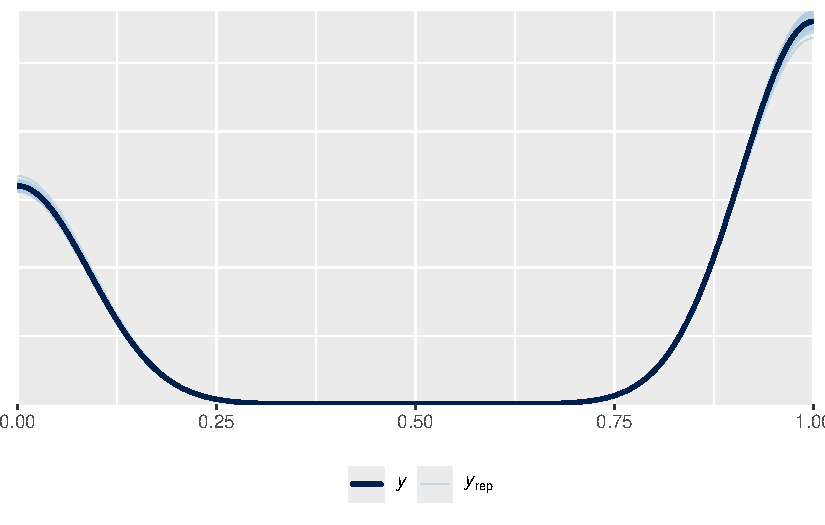
\includegraphics{paper_files/figure-pdf/fig-post_dist-1.pdf}

}

\caption{\label{fig-post_dist}Posterior distribution for logistic
regression model}

\end{figure}

\begin{figure}

\begin{minipage}[t]{0.50\linewidth}

{\centering 

\raisebox{-\height}{

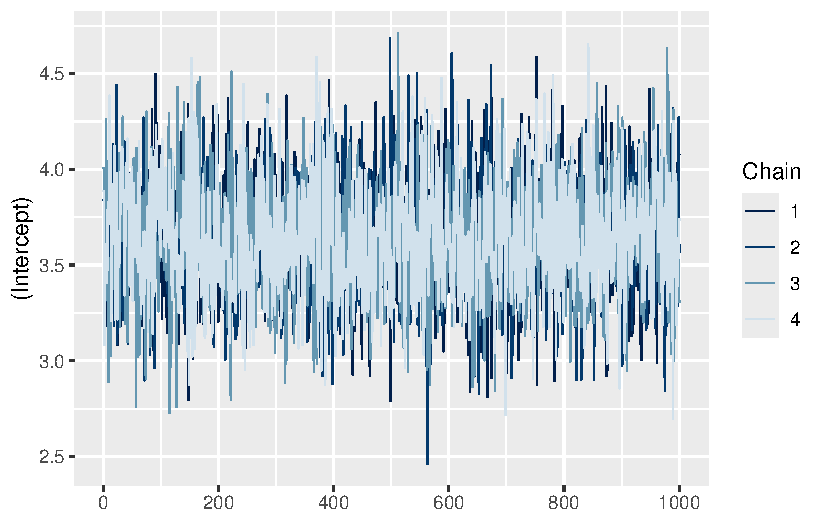
\includegraphics{paper_files/figure-pdf/fig-trace1-1.pdf}

}

}

\subcaption{\label{fig-trace1-1}Trace plot of Intercept}
\end{minipage}%
%
\begin{minipage}[t]{0.50\linewidth}

{\centering 

\raisebox{-\height}{

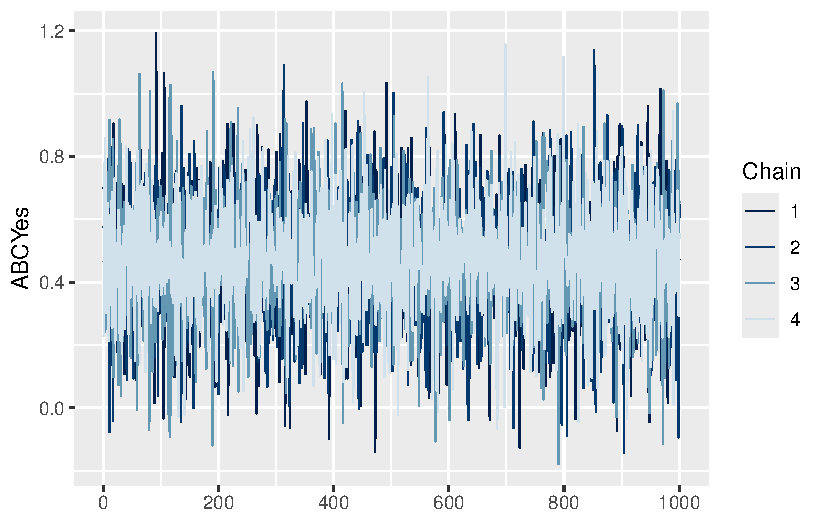
\includegraphics{paper_files/figure-pdf/fig-trace1-2.pdf}

}

}

\subcaption{\label{fig-trace1-2}Trace plot of race White}
\end{minipage}%
\newline
\begin{minipage}[t]{0.50\linewidth}

{\centering 

\raisebox{-\height}{

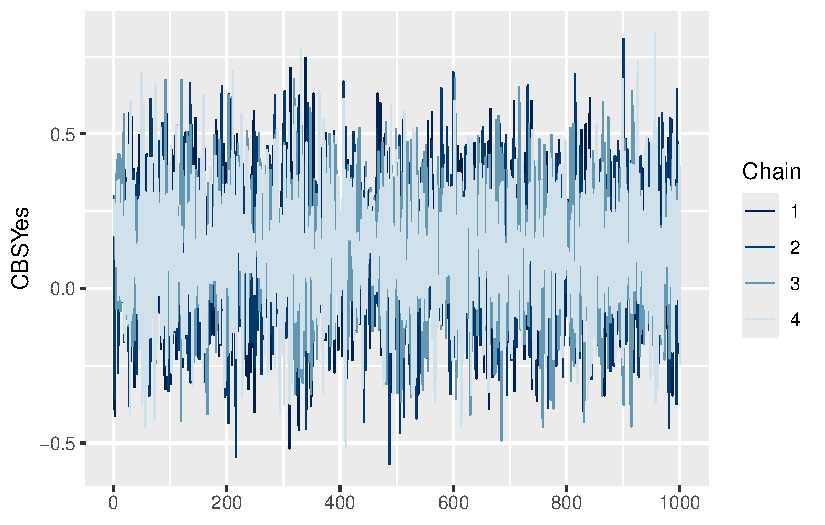
\includegraphics{paper_files/figure-pdf/fig-trace1-3.pdf}

}

}

\subcaption{\label{fig-trace1-3}Trace plot of race Black}
\end{minipage}%
%
\begin{minipage}[t]{0.50\linewidth}

{\centering 

\raisebox{-\height}{

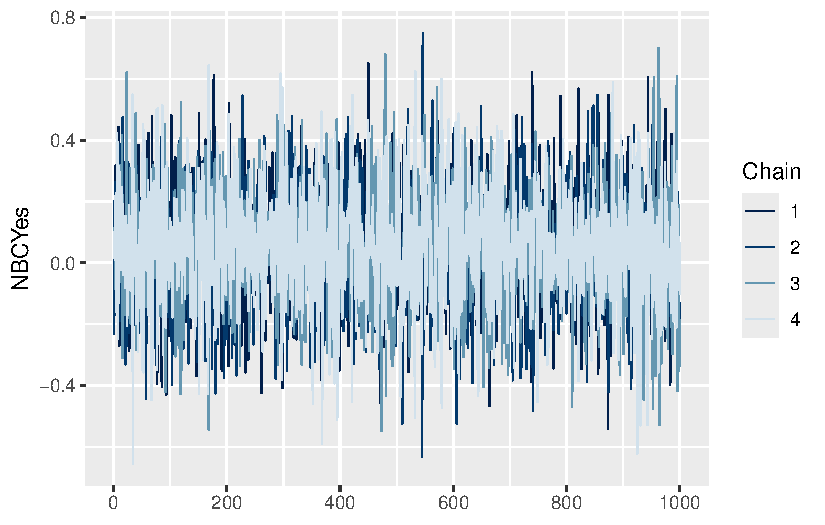
\includegraphics{paper_files/figure-pdf/fig-trace1-4.pdf}

}

}

\subcaption{\label{fig-trace1-4}Trace plot of race Hispanic}
\end{minipage}%
\newline
\begin{minipage}[t]{0.50\linewidth}

{\centering 

\raisebox{-\height}{

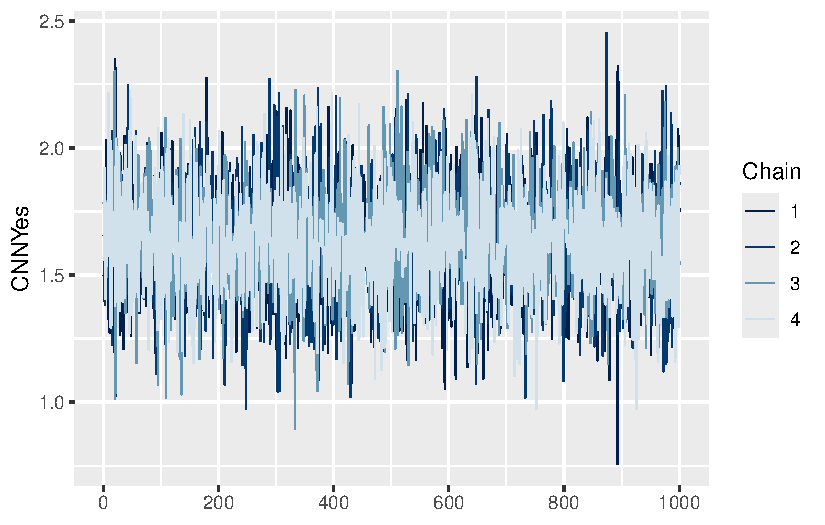
\includegraphics{paper_files/figure-pdf/fig-trace1-5.pdf}

}

}

\subcaption{\label{fig-trace1-5}Trace plot of race Middle Eastern}
\end{minipage}%
%
\begin{minipage}[t]{0.50\linewidth}

{\centering 

\raisebox{-\height}{

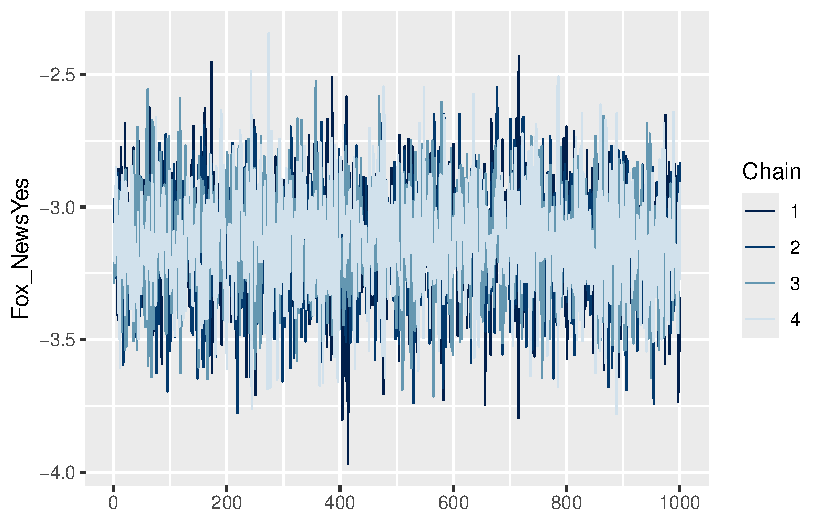
\includegraphics{paper_files/figure-pdf/fig-trace1-6.pdf}

}

}

\subcaption{\label{fig-trace1-6}Trace plot of race Native American}
\end{minipage}%
\newline
\begin{minipage}[t]{0.50\linewidth}

{\centering 

\raisebox{-\height}{

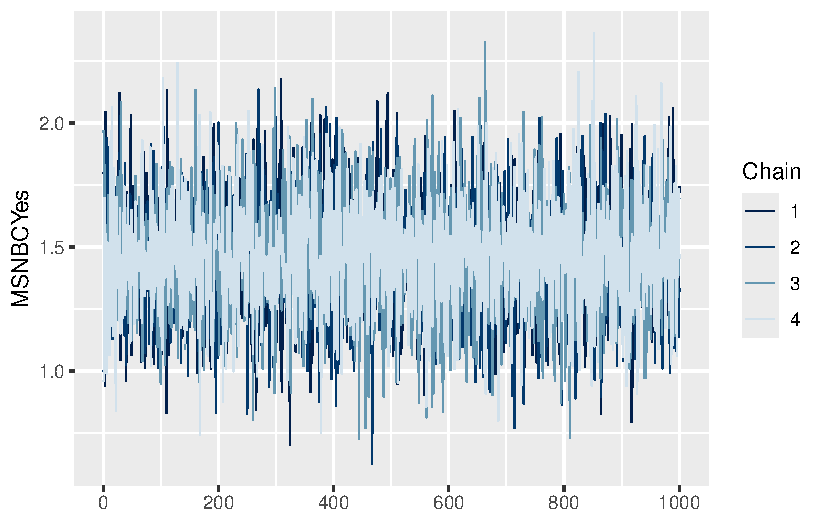
\includegraphics{paper_files/figure-pdf/fig-trace1-7.pdf}

}

}

\subcaption{\label{fig-trace1-7}Trace plot of race Two or more races}
\end{minipage}%
%
\begin{minipage}[t]{0.50\linewidth}

{\centering 

\raisebox{-\height}{

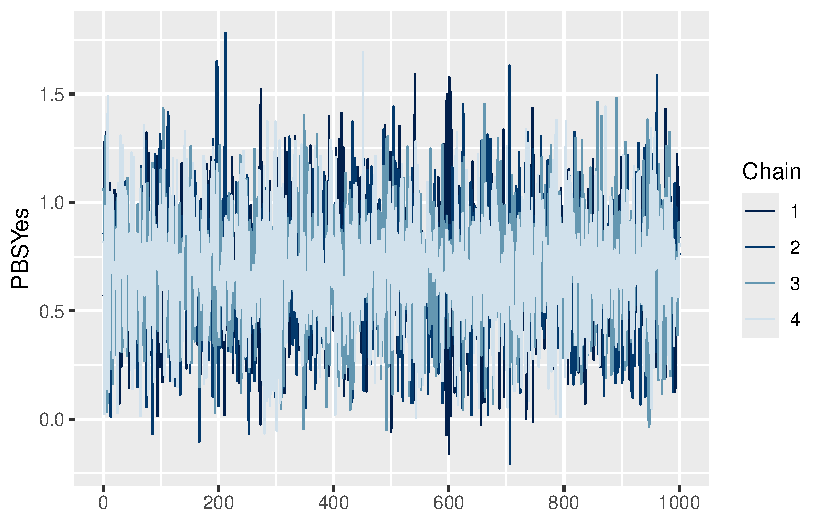
\includegraphics{paper_files/figure-pdf/fig-trace1-8.pdf}

}

}

\subcaption{\label{fig-trace1-8}Trace plot of race Other}
\end{minipage}%
\newline
\begin{minipage}[t]{0.50\linewidth}

{\centering 

\raisebox{-\height}{

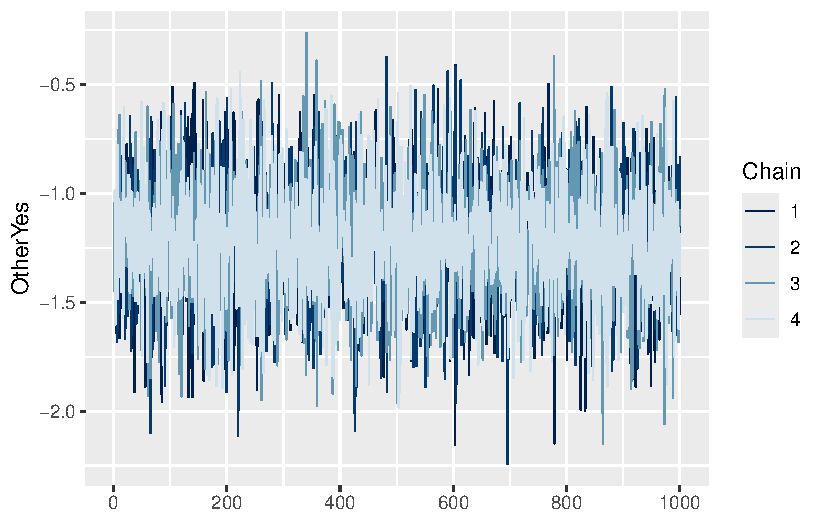
\includegraphics{paper_files/figure-pdf/fig-trace1-9.pdf}

}

}

\subcaption{\label{fig-trace1-9}Trace plot of Intercept}
\end{minipage}%

\caption{\label{fig-trace1}Trace plot of intercept and race}

\end{figure}

\begin{figure}

\begin{minipage}[t]{0.50\linewidth}

{\centering 

\raisebox{-\height}{

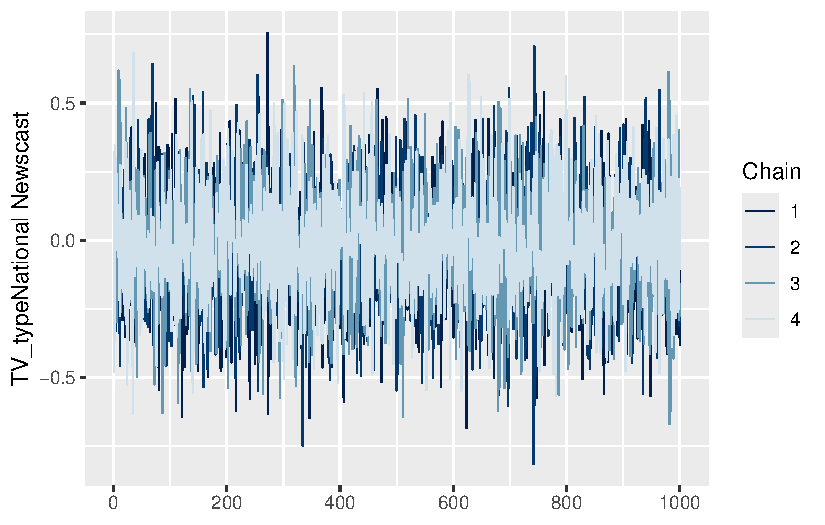
\includegraphics{paper_files/figure-pdf/fig-trace2-1.pdf}

}

}

\subcaption{\label{fig-trace2}Trace plot of region Northeast}
\end{minipage}%

\caption{\label{fig-trace2}Trace plot of region}

\end{figure}

\begin{figure}

\begin{minipage}[t]{0.50\linewidth}

{\centering 

\raisebox{-\height}{

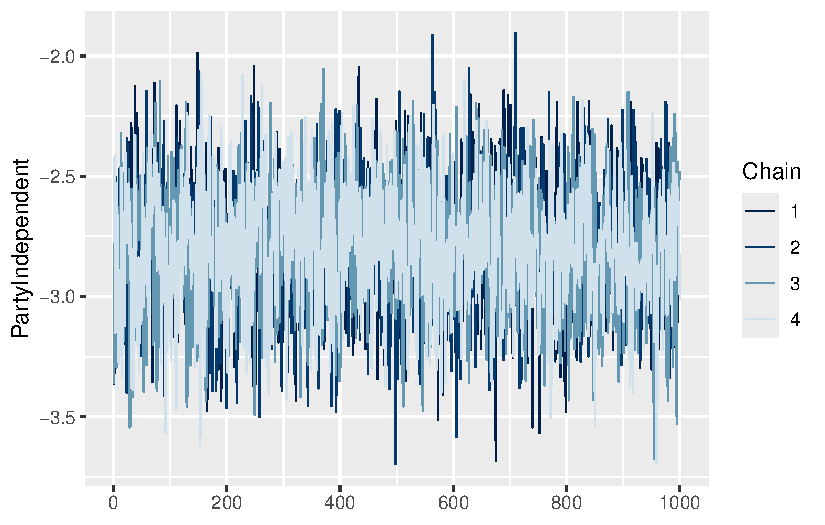
\includegraphics{paper_files/figure-pdf/fig-trace3-1.pdf}

}

}

\subcaption{\label{fig-trace3-1}Trace plot of region Northeast}
\end{minipage}%
%
\begin{minipage}[t]{0.50\linewidth}

{\centering 

\raisebox{-\height}{

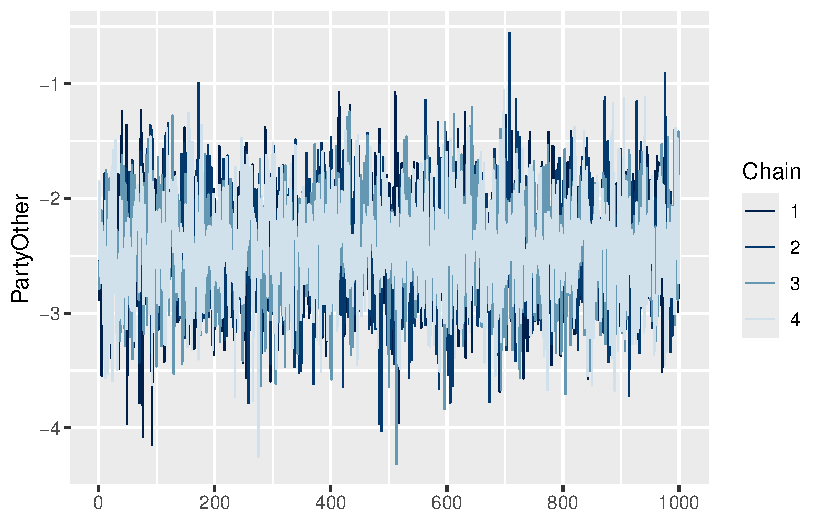
\includegraphics{paper_files/figure-pdf/fig-trace3-2.pdf}

}

}

\subcaption{\label{fig-trace3-2}Trace plot of region South}
\end{minipage}%
\newline
\begin{minipage}[t]{0.50\linewidth}

{\centering 

\raisebox{-\height}{

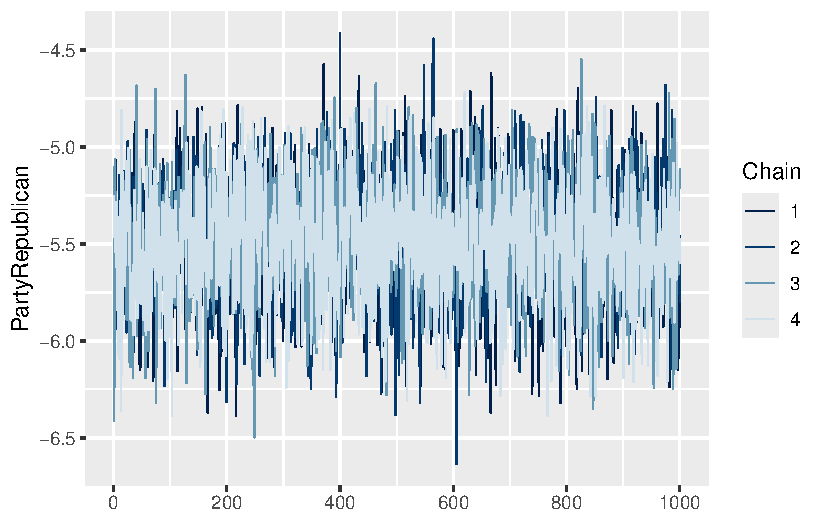
\includegraphics{paper_files/figure-pdf/fig-trace3-3.pdf}

}

}

\subcaption{\label{fig-trace3-3}Trace plot of region West}
\end{minipage}%

\caption{\label{fig-trace3}Trace plot of region}

\end{figure}

\begin{figure}

{\centering 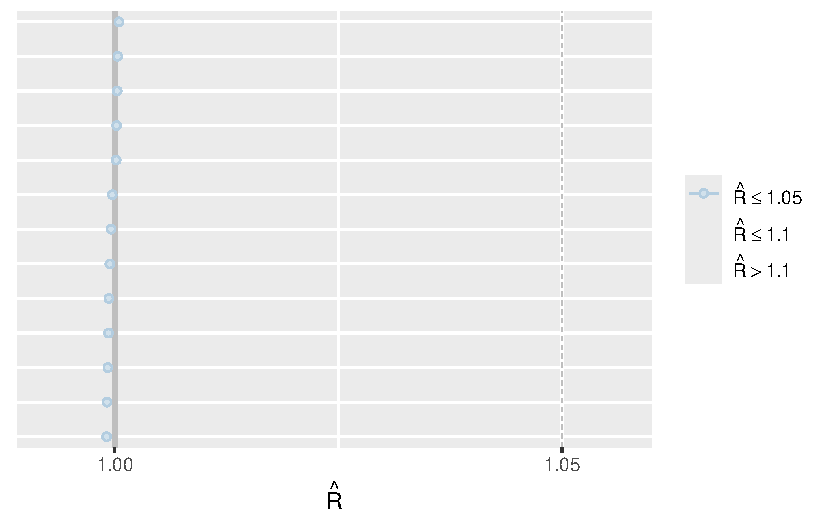
\includegraphics{paper_files/figure-pdf/fig-rhat-1.pdf}

}

\caption{\label{fig-rhat}Rhat plot}

\end{figure}

\hypertarget{sec-credibility-interval}{%
\subsection{Credibility Interval}\label{sec-credibility-interval}}

Figure~\ref{fig-modelresults1} shows the 90\% credibility interval for
the model.

\begin{figure}

{\centering 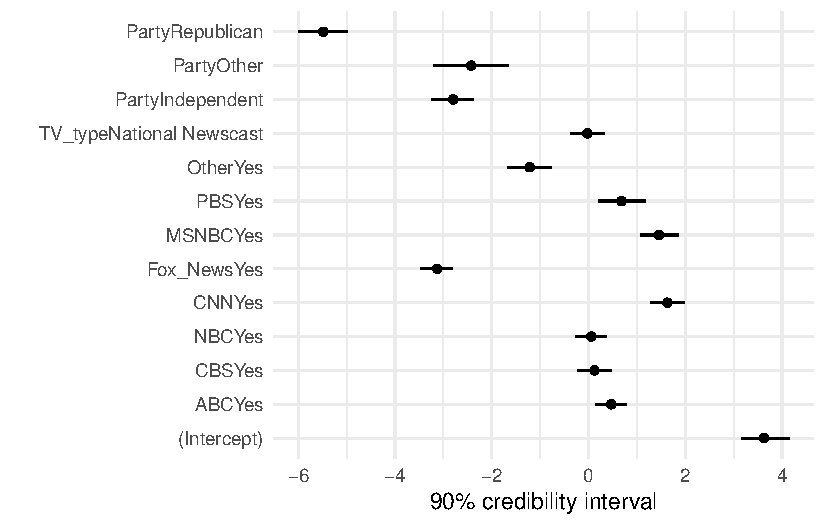
\includegraphics{paper_files/figure-pdf/fig-modelresults1-1.pdf}

}

\caption{\label{fig-modelresults1}Credible intervals for predictors of
support for Biden}

\end{figure}

\newpage

\hypertarget{references}{%
\section*{References}\label{references}}
\addcontentsline{toc}{section}{References}

\hypertarget{refs}{}
\begin{CSLReferences}{1}{0}
\leavevmode\vadjust pre{\hypertarget{ref-citeR}{}}%
R Core Team. 2023. \emph{R: A Language and Environment for Statistical
Computing}. Vienna, Austria: R Foundation for Statistical Computing.
\url{https://www.R-project.org/}.

\leavevmode\vadjust pre{\hypertarget{ref-rohan}{}}%
Wickham, Hadley, Mara Averick, Jennifer Bryan, Winston Chang, Lucy
D'Agostino McGowan, Romain François, Garrett Grolemund, et al. 2019.
{``Welcome to the {tidyverse}.''} \emph{Journal of Open Source Software}
4 (43): 1686. \url{https://doi.org/10.21105/joss.01686}.

\end{CSLReferences}



\end{document}
